\documentclass[12pt, a4paper]{article}

% --- Pakiety ---
\usepackage[utf8]{inputenc}
\usepackage[T1]{fontenc}
\usepackage[polish]{babel}
\usepackage{geometry}
\usepackage{amsmath}
\usepackage{amssymb}
\usepackage{graphicx}
\usepackage{booktabs}
\usepackage{siunitx}
\usepackage{caption}
\usepackage{subcaption}
\usepackage{float}
\usepackage{hyperref}
\usepackage{xcolor}
\usepackage{array}
\usepackage{multirow}
\usepackage{fancyhdr}

% --- Marginesy ---
\geometry{
    top=2.5cm,
    bottom=2.5cm,
    left=2.5cm,
    right=2.5cm,
    footskip=2cm
}

% --- Stopka ---
\pagestyle{fancy}
\fancyhf{}
\renewcommand{\headrulewidth}{0pt}
\renewcommand{\footrulewidth}{0.4pt}
\fancyfoot[R]{
\includegraphics[height=0.8cm]{lumon.pdf}}

% --- Konfiguracja siunitx ---
\sisetup{
    output-decimal-marker = {,},
    separate-uncertainty = true
}

% --- Dane raportu ---
\newcommand{\tytul}{Drgania tłumione i wymuszone tłumionego oscylatora harmonicznego}
\newcommand{\codeword}{Molde}
\newcommand{\nrCwiczenia}{M22}
\newcommand{\autor}{Karol Peszek}
\newcommand{\nrGrupy}{A}
\newcommand{\dataWykonania}{13 października 2026}

% --- Tytuł dokumentu ---
\title{
    \large I Pracownia Fizyczna \\[0.5em]
    \textbf{Ćwiczenie \nrCwiczenia} \\[0.3em]
    \LARGE \tytul\space''\codeword''
}
\author{
    \autor\\
     Grupa \nrGrupy}
\date{
    Data wykonania pomiarów: \dataWykonania\\
}

% =============================================
\begin{document}
% =============================================

\maketitle
\thispagestyle{empty}
\newpage

% -------------------------------------------
\section{Cel ćwiczenia}
% -------------------------------------------

W niniejszej pracy zbadano drgania swobodne, tłumione i wymuszone wahadła torsyjnego
(balansu) z~regulowanym hamulcem indukcyjnym. Wyznaczono częstość drgań własnych
wahadła $\omega_0$ oraz okresy drgań tłumionych dla siedmiu nastaw hamulca.
Z~zaniku amplitudy drgań tłumionych wyznaczono parametr tłumienia $\Gamma$ i~czas
relaksacji $\tau$ dla każdej nastawy. Wykonano kalibrację częstości siły wymuszającej
w~funkcji napięcia zasilania silnika, a następnie zmierzono krzywą rezonansową
i~dopasowano do niej model oscylatora wymuszonego, porównując otrzymane $\omega_0$
i~$\Gamma$ z~wartościami z~poprzednich części ćwiczenia.

% -------------------------------------------
\section{Wstęp teoretyczny}
% -------------------------------------------

\subsection{Wahadło torsyjne}

Wahadło torsyjne to bryła, której drgania powstają na skutek sił sprężystości ---
np.\ tarcza z~umocowaną do niej spiralną sprężyną. Skręcenie wahadła o~kąt $\varphi$
z~położenia równowagi prowadzi do powstania momentu siły sprężystości wprost
proporcjonalnego do wychylenia (prawo Hooke'a)~\cite{skrypt}:
\begin{equation}
    N_0 = -D_0\varphi,
    \label{eq:hooke}
\end{equation}
gdzie $D_0$ --- moment kierujący, zależny od parametrów sprężyny.
Równanie ruchu wahadła o~momencie bezwładności $J$ ma postać
\begin{equation}
    J\ddot{\varphi} + D_0\varphi = 0,
    \label{eq:harmonic}
\end{equation}
czyli jest równaniem oscylatora harmonicznego. Jego rozwiązaniem jest
$\varphi(t) = \varphi_0\cos(\omega_0 t + \delta)$, gdzie amplituda $\varphi_0$ i~faza
$\delta$ zależą od warunków początkowych, a
\begin{equation}
    \omega_0 = \frac{2\pi}{T_0} = \sqrt{\frac{D_0}{J}}
    \label{eq:omega0}
\end{equation}
jest częstością drgań własnych wahadła, $T_0$ --- okresem drgań swobodnych.

\subsection{Oscylator harmoniczny tłumiony}

Jeśli na wahadło działa dodatkowo moment siły hamującej wprost proporcjonalny do
prędkości kątowej, $N = -D\dot{\varphi}$, równanie ruchu przyjmuje postać~\cite{skrypt}:
\begin{equation}
    \ddot{\varphi} + \Gamma\dot{\varphi} + \omega_0^2\varphi = 0,
    \qquad \Gamma = \frac{D}{J},
    \label{eq:damped}
\end{equation}
gdzie $\Gamma$ --- parametr tłumienia. Taki moment wytwarza hamulec indukcyjny:
prądy wirowe indukowane w~metalowej tarczy poruszającej się w~polu elektromagnesu
hamują ją z~siłą proporcjonalną do jej prędkości kątowej, a~wartość $\Gamma$ reguluje
się natężeniem prądu płynącego przez uzwojenia elektromagnesu.

Dla tłumienia mniejszego od krytycznego, $\Gamma < \Gamma_\text{kr} = 2\omega_0$,
ruch jest oscylacyjny. Dla wahadła puszczonego z~wychylenia $\varphi_0$ z~zerową
prędkością kątową, $\varphi(0) = \varphi_0$, $\dot{\varphi}(0) = 0$, rozwiązanie
równania~\eqref{eq:damped} ma postać
\begin{equation}
    \varphi(t) = \varphi_0 e^{-\Gamma t/2}\left[\cos(\omega t)
                 + \frac{\Gamma}{2\omega}\sin(\omega t)\right],
    \label{eq:damped_solution}
\end{equation}
gdzie
\begin{equation}
    \omega = \frac{2\pi}{T} = \sqrt{\omega_0^2 - \left(\frac{\Gamma}{2}\right)^2}
    \label{eq:omega_damped}
\end{equation}
jest częstością drgań tłumionych, a $T$ --- ich okresem~\cite{skrypt}. Skrypt podaje
rozwiązanie w~przybliżonej postaci $\varphi_0 e^{-\Gamma t/2}\cos(\omega t)$, czyli
bez członu z~sinusem, który dla słabego tłumienia jest mały, ale jest potrzebny do
spełnienia warunku $\dot{\varphi}(0) = 0$. Częstość $\omega$ jest mniejsza
od $\omega_0$, przy czym dla słabego tłumienia ($\Gamma \ll \omega_0$) różnica jest
drugiego rzędu w~$\Gamma$: $\omega_0 - \omega \approx \Gamma^2/(8\omega_0)$.
Amplituda maleje wykładniczo (Rysunek~\ref{fig:damped_waveform}), a stała czasowa
\begin{equation}
    \tau = \frac{1}{\Gamma}
    \label{eq:tau}
\end{equation}
nazywana jest czasem relaksacji. Słabość tłumienia opisuje też \emph{dobroć}
oscylatora
\begin{equation}
    Q = \frac{\omega_0}{\Gamma} = \omega_0\tau.
    \label{eq:Q}
\end{equation}
Amplituda maleje $e$-krotnie po czasie $2\tau$, czyli po około $Q/\pi$ okresach.
Dla $\Gamma \geq \Gamma_\text{kr}$ wahadło nie
oscyluje, a przy tłumieniu krytycznym ($\Gamma = 2\omega_0$) wraca do położenia
równowagi najszybciej.

\begin{figure}[H]
    \centering
    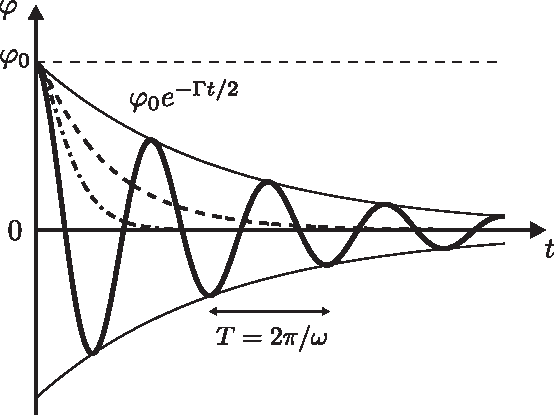
\includegraphics[width=0.55\textwidth]{suppressed_oscillations_waveform.pdf}
    \caption{Wychylenie oscylatora tłumionego $\varphi$ w~funkcji czasu dla wahadła
             puszczonego z~wychylenia $\varphi_0$ z~zerową prędkością kątową. Linia
             gruba --- słabe tłumienie $\Gamma < 2\omega_0$, cienkie linie --- obwiednia
             $\pm\varphi_0 e^{-\Gamma t/2}$, linia przerywana --- tłumienie krytyczne
             $\Gamma = 2\omega_0$ i~silne $\Gamma > 2\omega_0$.
             Źródło:~\cite{skrypt}.}\label{fig:damped_waveform}
\end{figure}

Prędkość kątowa wynikająca z~wzoru~\eqref{eq:damped_solution},
$\dot{\varphi}(t) = -\varphi_0\,(\omega_0^2/\omega)\,e^{-\Gamma t/2}\sin(\omega t)$,
zeruje się dokładnie w~chwilach $\omega t = (m-1)\pi$. Skrajne wychylenia wahadła
występują więc co pół okresu, w~chwilach $t_m = (m-1)\,T/2$, $m = 1, 2, \ldots$,
na przemian po stronie dodatniej i~ujemnej, i~leżą dokładnie na obwiedni:
\begin{equation}
    \varphi_m = (-1)^{m-1}\varphi_0\,e^{-\Gamma t_m/2}.
    \label{eq:extrema}
\end{equation}
Pomiar ciągu $\varphi_m$ pozwala więc wyznaczyć parametr tłumienia $\Gamma$.

\subsection{Oscylator wymuszony i~rezonans}

Jeśli na wahadło działa dodatkowo zewnętrzny moment siły $N_w(t)$, równanie ruchu
przyjmuje postać~\cite{skrypt}:
\begin{equation}
    \ddot{\varphi} + \Gamma\dot{\varphi} + \omega_0^2\varphi = f_0\cos(\Omega t),
    \label{eq:forced}
\end{equation}
gdzie $f_0\cos(\Omega t) = N_w(t)/J$ --- wymuszenie harmoniczne o~częstości $\Omega$.
Bezpośrednio po włączeniu wymuszenia lub zmianie jego częstości układ znajduje się
w~stanie nieustalonym. Po czasie znacznie dłuższym od czasu relaksacji $\tau$ osiąga
stan stacjonarny, w~którym drga z~częstością siły wymuszającej $\Omega$, niezależnie
od warunków początkowych (Rysunek~\ref{fig:forced}). W~stanie nieustalonym na drgania
wymuszone nakładają się drgania własne o~częstości $\omega \approx \omega_0$, zanikające
jak $e^{-\Gamma t/2}$. Ich suma daje \emph{dudnienia} --- amplituda okresowo rośnie
i~maleje z~okresem
\begin{equation}
    T_b = \frac{2\pi}{|\Omega - \omega_0|},
    \label{eq:beats}
\end{equation}
a~głębokość dudnień zmniejsza się w~miarę zaniku drgań własnych. Jeśli oscylator startuje
ze spoczynku w~położeniu równowagi, drgania własne mają na początku amplitudę bliską
amplitudzie stacjonarnej $\varphi_0$ i~fazę przeciwną, więc obwiednia dudnień zmienia się
od zera do $\varphi_0\,(1 + e^{-\Gamma t/2})$; maksima obwiedni wypadają w~chwilach
$t = T_b/2,\ 3T_b/2, \ldots$

\begin{figure}[H]
    \centering
    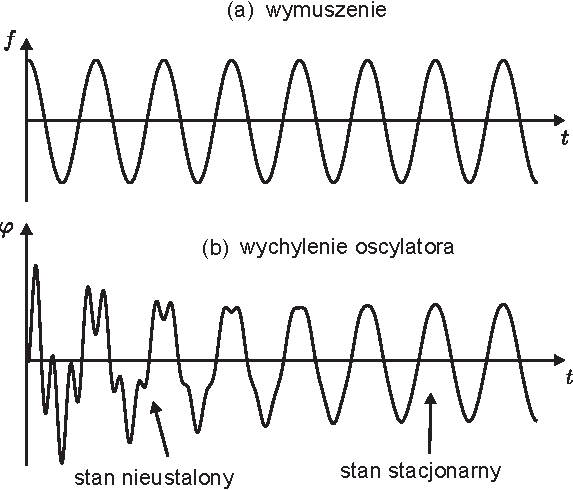
\includegraphics[width=0.55\textwidth]{forced_oscillations.pdf}
    \caption{Reakcja oscylatora tłumionego na wymuszenie sinusoidalne:
             (a)~wymuszenie $f$ w~funkcji czasu, (b)~wychylenie oscylatora $\varphi$
             w~funkcji czasu. Oscylator startuje z~położenia równowagi; po kilku
             okresach stanu nieustalonego przechodzi w~stan stacjonarny.
             Wykres dla $\Omega = 0{,}25\,\omega_0$ i~$\Gamma = 0{,}05\,\omega_0$.
             Źródło:~\cite{skrypt}.}\label{fig:forced}
\end{figure}

W~stanie stacjonarnym rozwiązaniem równania~\eqref{eq:forced} jest
$\varphi(t) = \varphi_0\cos(\Omega t - \delta)$, przy czym amplituda i~przesunięcie
fazowe względem wymuszenia wynoszą~\cite{skrypt}:
\begin{align}
    \varphi_0(\Omega) &= \frac{f_0}{\sqrt{(\omega_0^2 - \Omega^2)^2 + \Gamma^2\Omega^2}},
    \label{eq:resonance} \\
    \tan\delta &= \frac{\Gamma\Omega}{\omega_0^2 - \Omega^2}.
    \label{eq:phase}
\end{align}
W~pobliżu częstości drgań własnych amplituda wyraźnie rośnie i~osiąga maksimum ---
jest to zjawisko \emph{rezonansu}. Maksimum funkcji~\eqref{eq:resonance} występuje
dla częstości rezonansowej
\begin{equation}
    \omega_r = \sqrt{\omega_0^2 - \frac{\Gamma^2}{2}},
    \label{eq:omega_r}
\end{equation}
mniejszej od $\omega_0$; odchylenie rośnie wraz z~$\Gamma$. Im większe tłumienie,
tym krzywa rezonansowa jest niższa i~szersza (Rysunek~\ref{fig:resonance_theory}).
Dla słabego tłumienia amplituda w~rezonansie,
$\varphi_0(\omega_r) \approx f_0/(\Gamma\omega_0)$, jest około $Q$~razy większa
od wychylenia przy wymuszeniu statycznym, $\varphi_0(0) = f_0/\omega_0^2$.
Dla słabego tłumienia jej szerokość połówkowa (mierzona w~połowie wysokości) jest
rzędu $\sqrt{3}\,\Gamma$. Przesunięcie fazowe~\eqref{eq:phase} zmienia się od $0$
dla małych częstości, przez $90^{\circ}$ dla $\Omega = \omega_0$, do $180^{\circ}$
(przeciwfaza) dla dużych częstości.

\begin{figure}[H]
    \centering
    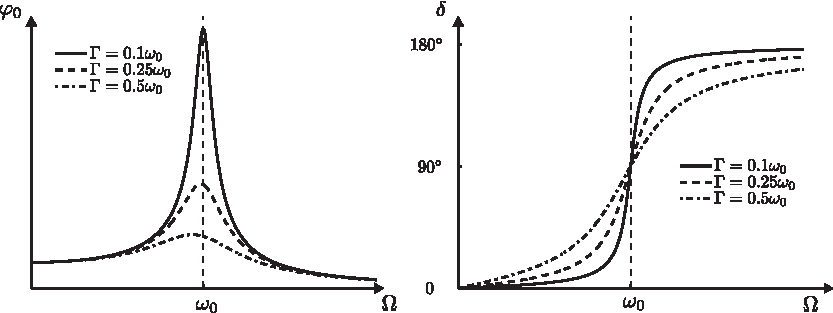
\includegraphics[width=0.95\textwidth]{resonance_curve_diagram.pdf}
    \caption{Amplituda $\varphi_0$ (lewy wykres, krzywe rezonansowe) i~przesunięcie
             fazowe $\delta$ (prawy wykres) drgań stacjonarnych oscylatora w~funkcji
             częstości wymuszenia $\Omega$ dla trzech wartości parametru tłumienia
             $\Gamma$. Źródło:~\cite{skrypt}.}\label{fig:resonance_theory}
\end{figure}



% -------------------------------------------
\section{Opis układu pomiarowego}
% -------------------------------------------

Układ pomiarowy przedstawiono na Rysunku~\ref{fig:setup_photo}. Jego głównym elementem
jest wahadło torsyjne typu balans --- miedziana tarcza osadzona na osi, połączona
ze spiralną sprężyną taśmową (Rysunek~\ref{fig:pendulum}). Wychylenie odczytuje się
na kołowej skali za pomocą wskazówki zamocowanej do tarczy.

\begin{figure}[H]
    \centering
    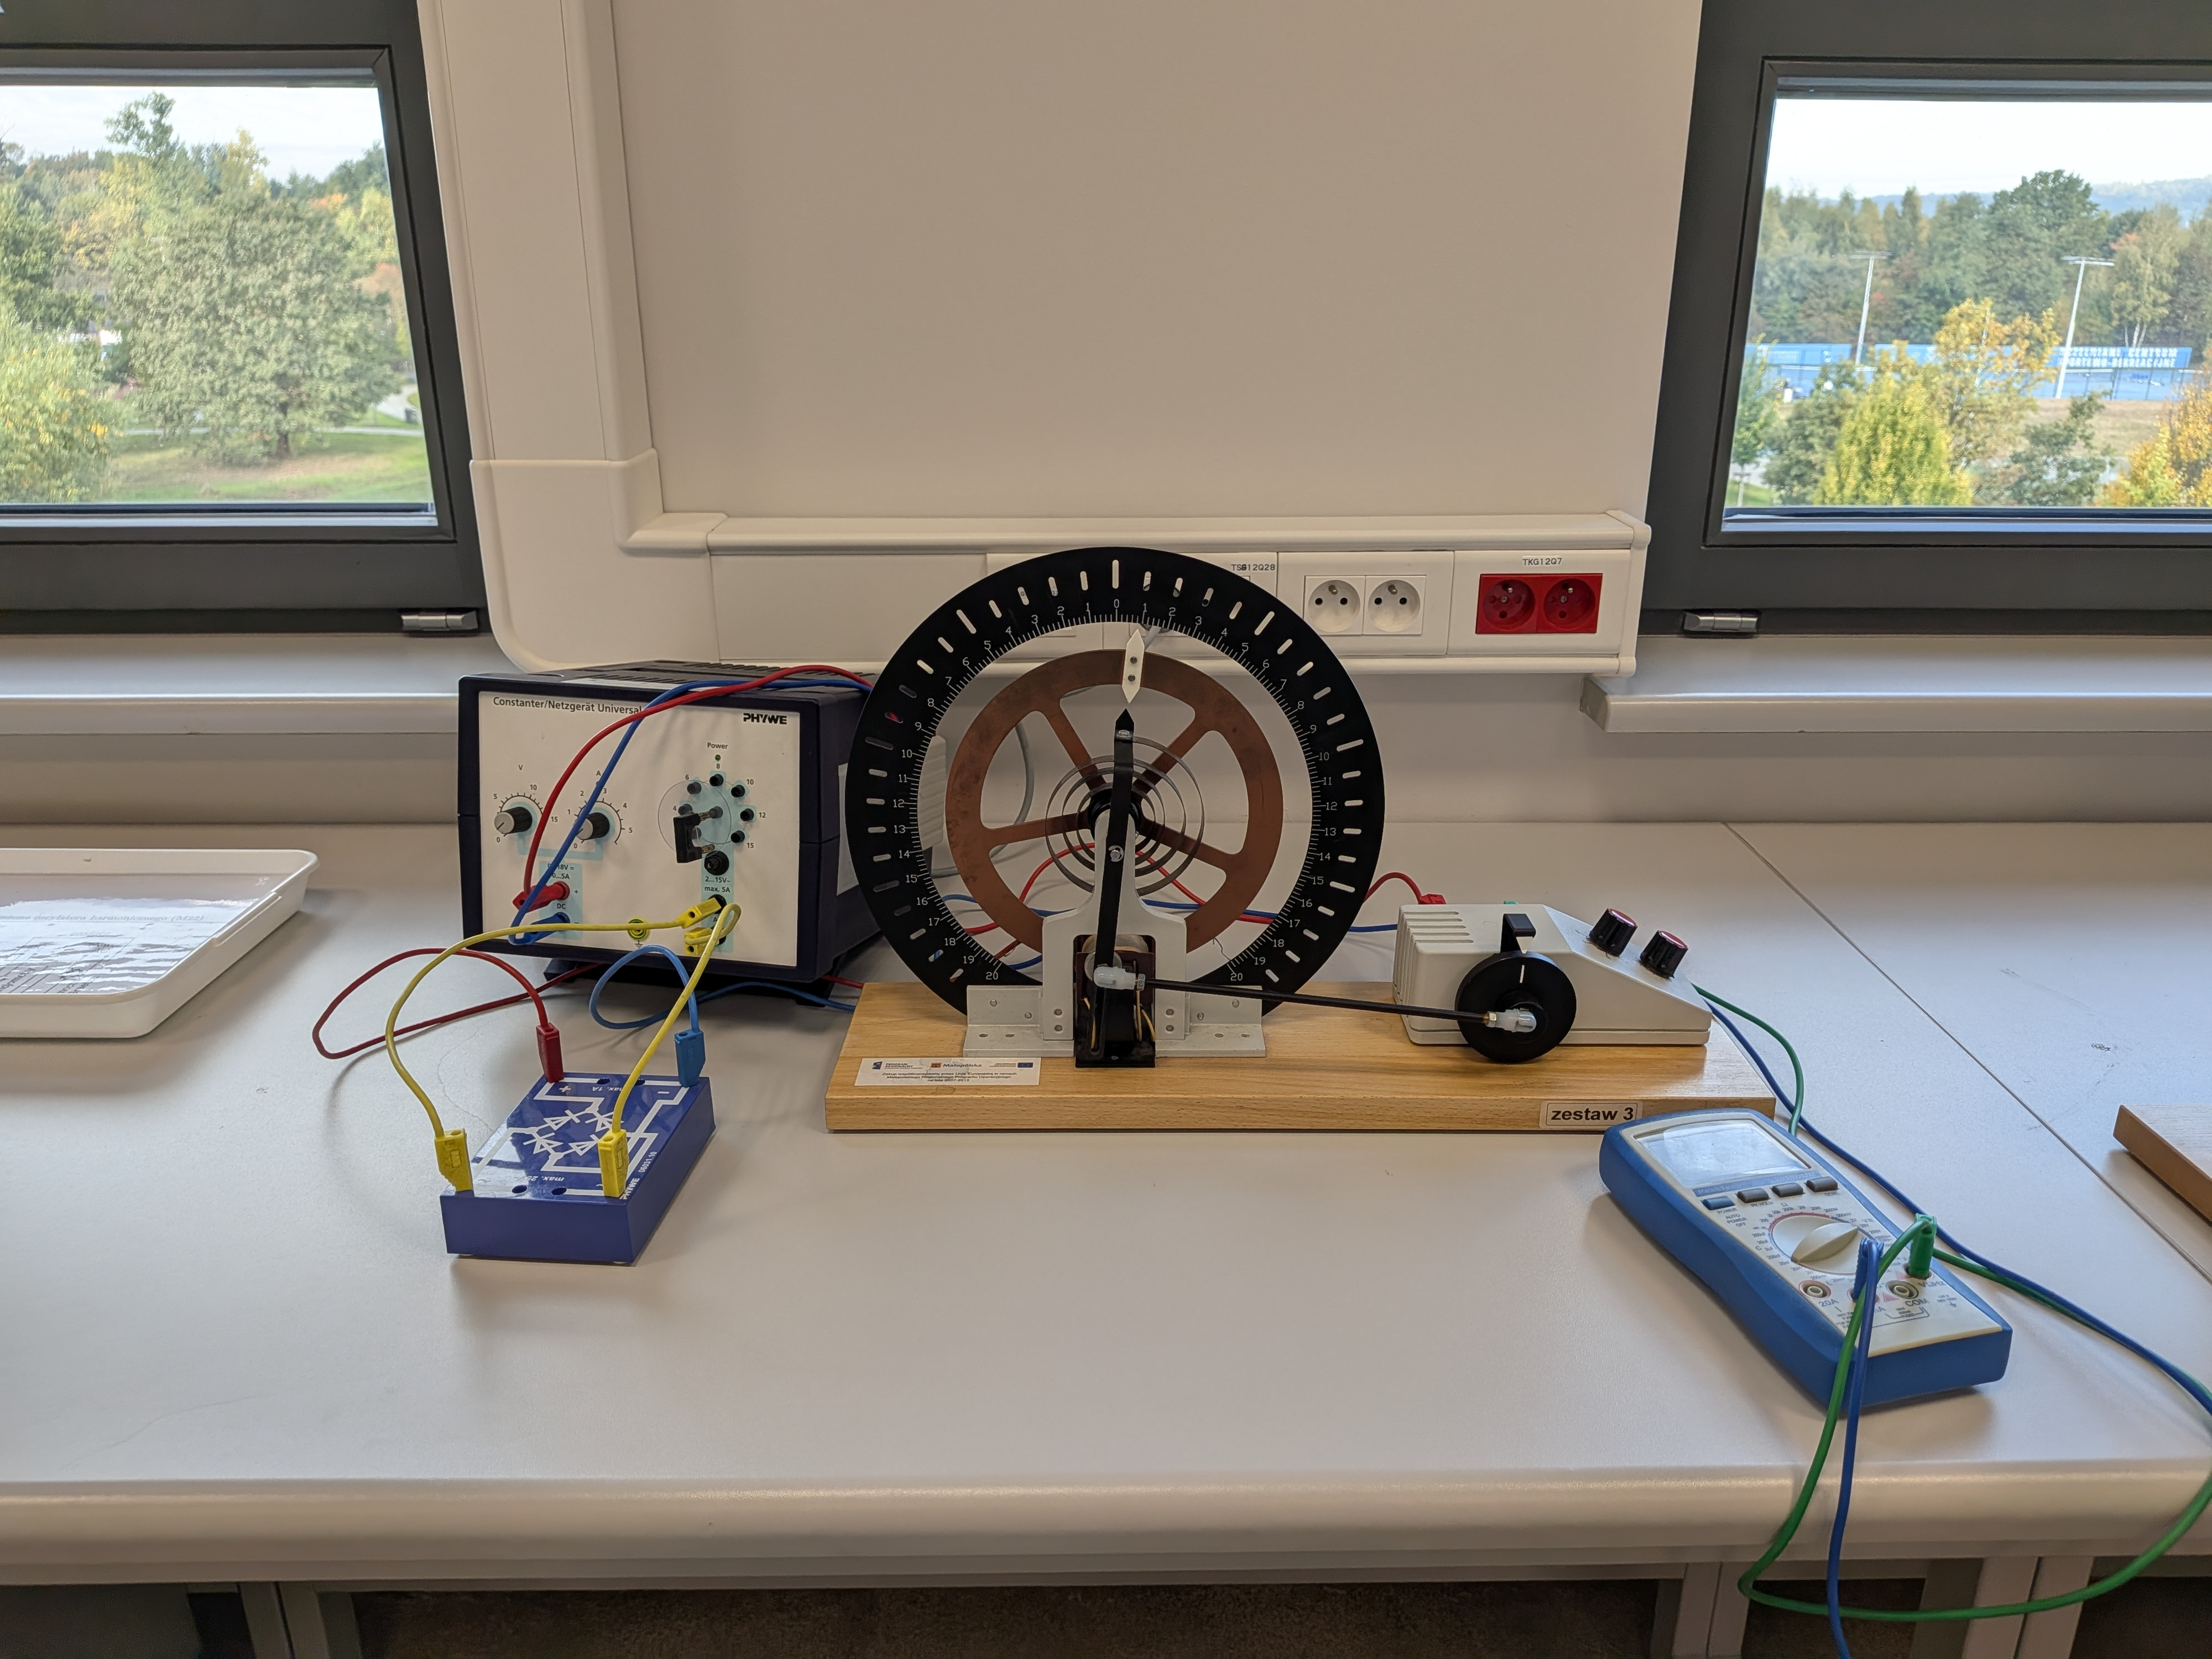
\includegraphics[width=0.82\textwidth]{schema.jpg}
    \caption{Układ pomiarowy. Od lewej: zasilacz z~pokrętłem Power, mostek Graetza,
             wahadło balansowe ze skalą, silnik wymuszający z~potencjometrami,
             multimetr mierzący napięcie zasilania silnika.}\label{fig:setup_photo}
\end{figure}

\begin{figure}[H]
    \centering
    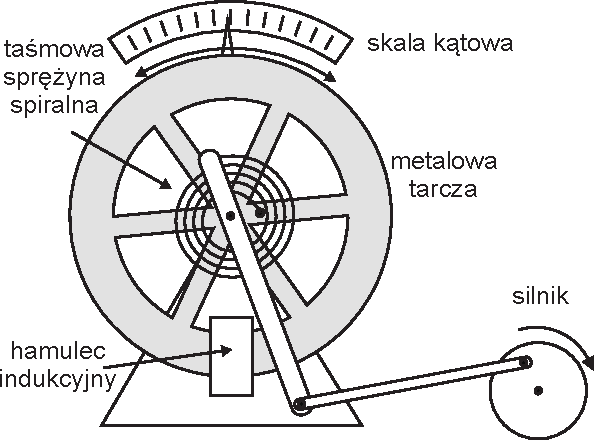
\includegraphics[width=0.55\textwidth]{schema.pdf}
    \caption{Budowa wahadła balansowego: metalowa tarcza ze spiralną sprężyną taśmową,
             skala kątowa, hamulec indukcyjny i~silnik połączony z~wahadłem
             mimośrodowo. Źródło:~\cite{skrypt}.}\label{fig:pendulum}
\end{figure}

W skład układu wchodzą:
\begin{itemize}
    \item wahadło balansowe ze skalą w~jednostkach umownych [j.u.], opisaną od $0$
          do $20$ po obu stronach położenia równowagi (pełne $180^{\circ}$ odpowiada
          około $25$~j.u.);
    \item hamulec indukcyjny --- elektromagnes, między którego nabiegunnikami porusza
          się brzeg tarczy; tłumienie reguluje się prądem uzwojeń za pomocą pokrętła
          Power na zasilaczu (nastawy w~jednostkach umownych);
    \item silnik prądu stałego z~mimośrodem, połączony prętami ze sprężyną wahadła,
          wytwarzający okresowy moment wymuszający; częstość wymuszenia reguluje się
          napięciem zasilania silnika za pomocą dwóch potencjometrów (zgrubnego
          i~dokładnego);
    \item zasilacz PHYWE z~wyjściem stałonapięciowym (silnik) i~zmiennonapięciowym
          (hamulec) oraz mostek Graetza prostujący prąd hamulca;
    \item multimetr PeakTech 2010 DMM w~trybie woltomierza, mierzący napięcie
          zasilania silnika $U$; ze względu na wahania wskazania przyjęto
          $u_U = \SI{0.1}{\volt}$;
    \item stoper o~rozdzielczości \SI{0.01}{\second}; jako niepewność pojedynczego
          pomiaru czasu przyjęto czas reakcji człowieka, $u_T = \SI{0.3}{\second}$;
    \item kamera telefonu, którą nagrywano drgania tłumione w~celu odczytu kolejnych
          wychyleń z~nagrania.
\end{itemize}

Połączenia wykonano zgodnie ze schematem ze skryptu~\cite{skrypt}: wyjście
stałonapięciowe zasilacza zasila przez potencjometry silnik, równolegle do którego
podłączono woltomierz, a~wyjście zmiennonapięciowe przez mostek Graetza zasila
elektromagnes hamulca.

% -------------------------------------------
\section{Procedura pomiarowa}
% -------------------------------------------

\subsection{Kalibracja częstości siły wymuszającej}\label{sec:proc_calibration}

Zmierzono okres obrotu mimośrodu silnika, równy okresowi siły wymuszającej,
w~funkcji napięcia zasilania silnika. Dla $11$~napięć
zasilania silnika z~zakresu \SIrange{1.77}{15.02}{\volt} zmierzono stoperem czas
$5$~pełnych obrotów (dla $U \leq \SI{8.68}{\volt}$) lub $10$~obrotów (dla wyższych
napięć, przy których obrót jest krótszy). Każdy pomiar czasu powtórzono trzykrotnie.

\subsection{Drgania swobodne}\label{sec:proc_free}

Przy wyłączonym hamulcu i~silniku wahadło wychylono do maksymalnego wychylenia
i~puszczono z~zerową prędkością. Zmierzono czas $5$~pełnych okresów drgań;
pomiar powtórzono $10$~razy.

\subsection{Okresy drgań tłumionych}\label{sec:proc_damped_periods}

Dla siedmiu nastaw hamulca Power: $2$, $4$, $6$, $8$, $10$, $12$ i~$15$ wahadło
puszczano z~maksymalnego wychylenia i~mierzono czas $5$~okresów drgań.
Dla każdej nastawy pomiar wykonano trzykrotnie.

\subsection{Zanik amplitudy drgań tłumionych}\label{sec:proc_decay}

Dla tych samych siedmiu nastaw hamulca wahadło puszczano z~maksymalnego
wychylenia (około $19$~j.u.) i~nagrywano jego ruch kamerą. Z~nagrania odczytano
$12$~kolejnych skrajnych wychyleń $\varphi_m$, na przemian po stronie dodatniej
i~ujemnej, czyli co pół okresu, począwszy od pierwszego ekstremum po puszczeniu
wahadła ($\varphi_1$, pół okresu po starcie; por.\ Sekcja~\ref{sec:op_decay}).
Dla każdej nastawy wykonano trzy serie.

\subsection{Krzywa rezonansowa}\label{sec:proc_resonance}

Krzywą rezonansową zmierzono dla nastawy hamulca Power~$=6$. Napięcie zasilania
silnika ustawiano kolejno na $8$~wartości z~zakresu \SIrange{3.85}{13.51}{\volt},
zagęszczając pomiary w~okolicy rezonansu (\SIrange{7.11}{8.80}{\volt}).
Precyzyjną zmianę napięcia uzyskiwano potencjometrem dokładnym. Po każdej zmianie
napięcia wahadło zatrzymywano ręcznie w~położeniu równowagi, zgodnie z~zaleceniem
skryptu~\cite{skrypt}, więc rozpędzało się praktycznie od zera. W~wyniku takiego startu
w~ruchu wahadła występowały dudnienia --- amplituda okresowo rosła i~malała.
Obserwowano, kiedy następuje największe wychylenie, i~czekano na kolejne maksimum
dudnień, w~którym odczytywano skrajne wychylenia wahadła $\varphi_-$ i~$\varphi_+$.
Nie czekano na pełny zanik dudnień, więc odczytane wartości odpowiadają maksimum
dudnień, a~nie ściśle stanowi stacjonarnemu.



% -------------------------------------------
\section{Wyniki pomiarów}
% -------------------------------------------

We wszystkich pomiarach niepewność pojedynczego pomiaru czasu wynosi
$u_T = \SI{0.3}{\second}$, niepewność napięcia zasilania silnika $u_U = \SI{0.1}{\volt}$,
a~niepewność odczytu wychylenia $u_A = 0{,}2$~j.u.\ przy odczycie z~nagrania
(zanik amplitudy) i~$u_A = 0{,}6$~j.u.\ przy odczycie bezpośrednim (krzywa rezonansowa).

\subsection{Kalibracja częstości siły wymuszającej}\label{sec:res_calibration}

Zmierzone czasy $n$~obrotów silnika zestawiono w~Tabeli~\ref{tab:calibration_raw},
a~odpowiadające im częstości wymuszenia $\Omega = 2\pi n/\overline{t}$, gdzie
$\overline{t}$ --- średnia z~trzech pomiarów, przedstawiono na
Rysunku~\ref{fig:calibration_raw}.

\begin{table}[H]
    \centering
    \caption{Czasy $t_1$, $t_2$, $t_3$ trzech pomiarów $n$~obrotów silnika
             w~funkcji napięcia zasilania $U$. Niepewności: $u_U = \SI{0.1}{\volt}$,
             $u_T = \SI{0.3}{\second}$.}\label{tab:calibration_raw}
    \begin{tabular}{S[table-format=2.2] S[table-format=2.0]
                    S[table-format=2.2] S[table-format=2.2] S[table-format=2.2]}
        \toprule
        {$U$ [V]} & {$n$} & {$t_1$ [s]} & {$t_2$ [s]} & {$t_3$ [s]} \\
        \midrule
        1.77 & 5 & 54.09 & 54.44 & 54.16 \\
        2.64 & 5 & 30.30 & 30.55 & 30.13 \\
        3.67 & 5 & 20.74 & 20.87 & 20.39 \\
        5.60 & 5 & 12.30 & 12.24 & 12.23 \\
        6.91 & 5 & 10.04 & 10.19 & 10.13 \\
        8.68 & 5 & 7.69 & 7.75 & 7.73 \\
        9.73 & 10 & 13.82 & 13.79 & 13.94 \\
        11.44 & 10 & 11.80 & 11.89 & 11.88 \\
        12.67 & 10 & 10.59 & 10.65 & 10.45 \\
        14.41 & 10 & 9.30 & 9.34 & 9.39 \\
        15.02 & 10 & 8.91 & 8.99 & 9.10 \\
        \bottomrule
    \end{tabular}
\end{table}

\begin{figure}[H]
    \centering
    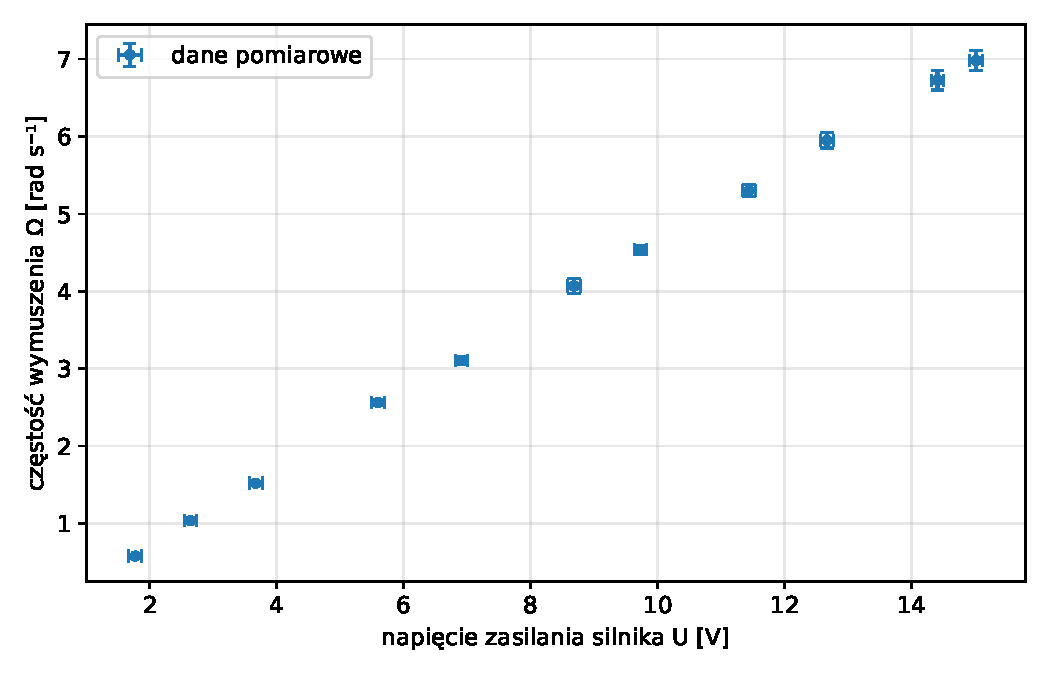
\includegraphics[width=0.82\textwidth]{force_calibration_raw.pdf}
    \caption{Częstość siły wymuszającej $\Omega$ w~funkcji napięcia zasilania
             silnika $U$. Słupki błędów odpowiadają niepewnościom $u_U = \SI{0.1}{\volt}$
             i~$u(\Omega)$ wynikającej z~niepewności pomiaru czasu.}\label{fig:calibration_raw}
\end{figure}

\subsection{Drgania swobodne}\label{sec:res_free}

Wyniki dziesięciu pomiarów czasu $5T_0$ zestawiono w~Tabeli~\ref{tab:free_raw},
a~odpowiadające im okresy $T_0$ przedstawiono na Rysunku~\ref{fig:free_raw}.

\begin{table}[H]
    \centering
    \caption{Czasy pięciu okresów drgań swobodnych $5T_0$ w~kolejnych pomiarach.
             Niepewność każdego pomiaru $u_T = \SI{0.3}{\second}$.}\label{tab:free_raw}
    \begin{tabular}{l *{10}{S[table-format=1.2]}}
        \toprule
        nr pomiaru & {1} & {2} & {3} & {4} & {5} & {6} & {7} & {8} & {9} & {10} \\
        \midrule
        $5T_0$ [s] & 8.87 & 8.99 & 8.83 & 8.87 & 8.94 & 8.84 & 8.94 & 8.86 & 8.73 & 8.81 \\
        \bottomrule
    \end{tabular}
\end{table}

\begin{figure}[H]
    \centering
    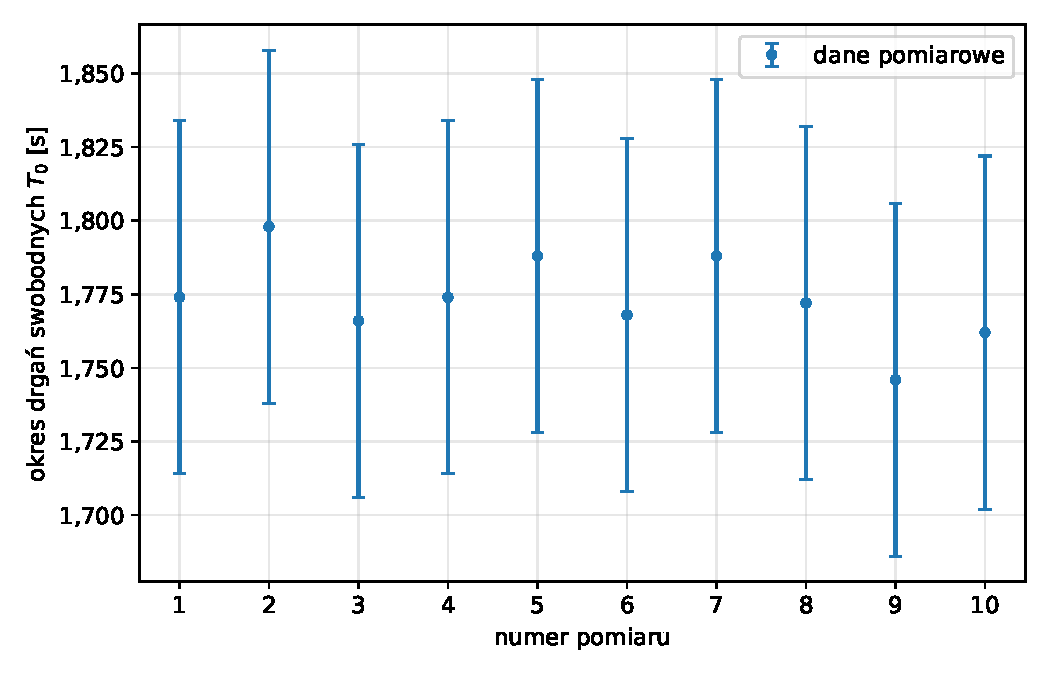
\includegraphics[width=0.82\textwidth]{free_oscillations_raw.pdf}
    \caption{Okres drgań swobodnych $T_0$ w~kolejnych pomiarach. Słupki błędów
             odpowiadają niepewności $u_T/5 = \SI{0.06}{\second}$.}\label{fig:free_raw}
\end{figure}

\subsection{Okresy drgań tłumionych}\label{sec:res_damped_periods}

Czasy pięciu okresów drgań tłumionych dla kolejnych nastaw hamulca zestawiono
w~Tabeli~\ref{tab:damped_periods_raw}, a~średnie okresy $T$ przedstawiono na
Rysunku~\ref{fig:damped_periods_raw}.

\begin{table}[H]
    \centering
    \caption{Czasy $t_1$, $t_2$, $t_3$ trzech pomiarów pięciu okresów drgań tłumionych
             dla kolejnych nastaw hamulca Power. Niepewność każdego pomiaru
             $u_T = \SI{0.3}{\second}$.}\label{tab:damped_periods_raw}
    \begin{tabular}{S[table-format=2.0] S[table-format=1.2] S[table-format=1.2] S[table-format=1.2]}
        \toprule
        {Power [j.u.]} & {$t_1$ [s]} & {$t_2$ [s]} & {$t_3$ [s]} \\
        \midrule
        2 & 8.87 & 8.81 & 8.93 \\
        4 & 8.88 & 8.94 & 8.88 \\
        6 & 8.92 & 8.98 & 8.90 \\
        8 & 8.93 & 9.01 & 9.02 \\
        10 & 9.02 & 8.87 & 8.97 \\
        12 & 9.01 & 8.87 & 8.88 \\
        15 & 8.84 & 8.87 & 8.80 \\
        \bottomrule
    \end{tabular}
\end{table}

\begin{figure}[H]
    \centering
    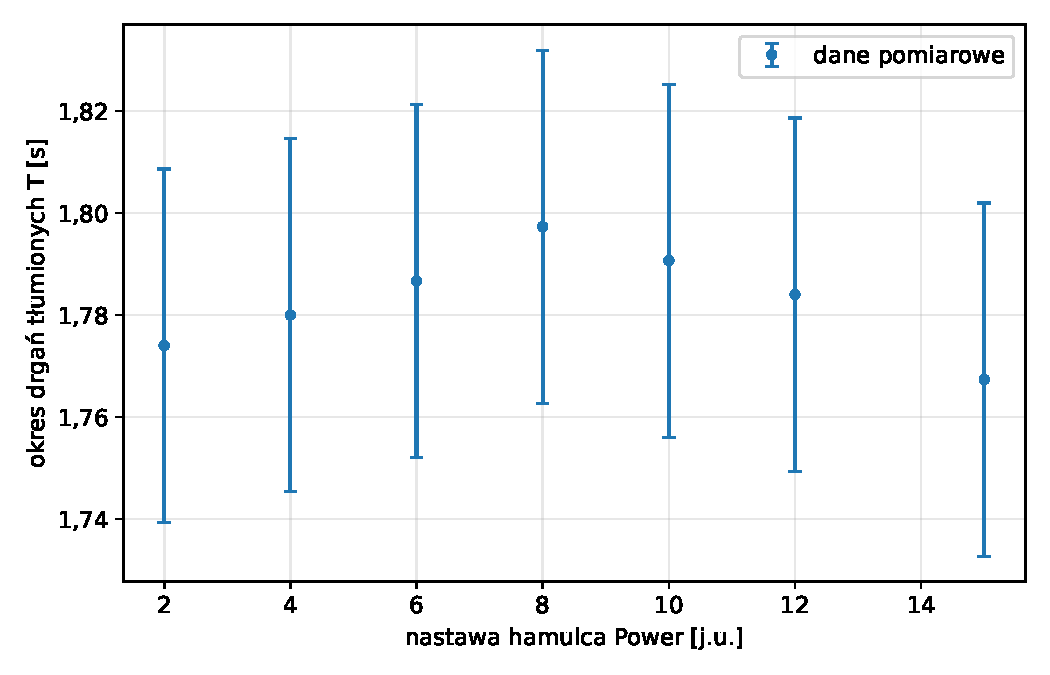
\includegraphics[width=0.82\textwidth]{damped_periods_raw.pdf}
    \caption{Średni okres drgań tłumionych $T$ w~funkcji nastawy hamulca. Słupki
             błędów odpowiadają niepewności średniej z~trzech pomiarów,
             $u(T) = u_T/(5\sqrt{3}) \approx \SI{0.035}{\second}$.}\label{fig:damped_periods_raw}
\end{figure}

\subsection{Zanik amplitudy drgań tłumionych}\label{sec:res_decay}

Kolejne skrajne wychylenia wahadła odczytane z~nagrań zestawiono
w~Tabeli~\ref{tab:decay_raw}. Na Rysunku~\ref{fig:decay_raw} przedstawiono je
w~funkcji czasu $t_m = (m-1)\,T/2$ osobno dla każdej nastawy hamulca,
a~na Rysunku~\ref{fig:envelope_raw} --- moduły wychyleń uśrednione po trzech
seriach, dla wszystkich nastaw na jednym wykresie.

\begin{table}[H]
    \centering
    \caption{Kolejne skrajne wychylenia wahadła $\varphi_m$ [j.u.] w~trzech seriach
             dla każdej nastawy hamulca Power. Niepewność odczytu
             $u_A = 0{,}2$~j.u.}\label{tab:decay_raw}
    \resizebox{\textwidth}{!}{%
    \begin{tabular}{c c *{12}{S[table-format=-2.1]}}
        \toprule
        {Power} & {seria} & {$\varphi_1$} & {$\varphi_2$} & {$\varphi_3$} & {$\varphi_4$}
        & {$\varphi_5$} & {$\varphi_6$} & {$\varphi_7$} & {$\varphi_8$} & {$\varphi_9$}
        & {$\varphi_{10}$} & {$\varphi_{11}$} & {$\varphi_{12}$} \\
        \midrule
        \multirow{3}{*}{2} & 1 & 19.0 & -18.8 & 18.4 & -18.4 & 17.8 & -17.8 & 17.4 & -17.2 & 16.8 & -16.6 & 16.2 & -16.2 \\
         & 2 & 19.0 & -19.0 & 18.4 & -18.6 & 18.0 & -18.0 & 17.4 & -17.4 & 17.0 & -17.0 & 16.4 & -16.4 \\
         & 3 & 18.8 & -18.8 & 18.2 & -18.2 & 17.8 & -17.8 & 17.2 & -17.2 & 16.6 & -16.6 & 16.2 & -16.2 \\
        \midrule
        \multirow{3}{*}{4} & 1 & 19.0 & -18.8 & 18.2 & -18.0 & 17.6 & -17.4 & 17.0 & -16.8 & 16.2 & -16.2 & 15.6 & -15.4 \\
         & 2 & 18.8 & -18.6 & 18.0 & -18.0 & 17.4 & -17.4 & 16.8 & -16.8 & 16.2 & -16.0 & 15.6 & -15.4 \\
         & 3 & 18.8 & -18.6 & 18.0 & -18.0 & 17.4 & -17.2 & 16.6 & -16.6 & 16.0 & -15.8 & 15.2 & -15.0 \\
        \midrule
        \multirow{3}{*}{6} & 1 & 18.8 & -18.4 & 17.8 & -17.6 & 16.8 & -16.6 & 16.0 & -15.8 & 15.0 & -14.8 & 14.2 & -14.0 \\
         & 2 & 18.8 & -18.4 & 17.8 & -17.4 & 16.8 & -16.6 & 16.0 & -15.6 & 15.2 & -15.0 & 14.4 & -14.0 \\
         & 3 & 18.8 & -18.4 & 17.6 & -17.4 & 17.0 & -16.4 & 16.0 & -15.8 & 15.0 & -15.0 & 14.2 & -14.0 \\
        \midrule
        \multirow{3}{*}{8} & 1 & 18.6 & -18.0 & 17.0 & -16.4 & 15.8 & -15.2 & 14.4 & -14.0 & 13.4 & -13.0 & 12.2 & -11.8 \\
         & 2 & 18.6 & -18.0 & 17.2 & -16.8 & 15.8 & -15.4 & 14.6 & -14.2 & 13.4 & -13.0 & 12.4 & -12.0 \\
         & 3 & 18.6 & -18.0 & 17.0 & -16.6 & 15.8 & -15.4 & 14.6 & -14.2 & 13.6 & -13.2 & 12.4 & -12.0 \\
        \midrule
        \multirow{3}{*}{10} & 1 & 18.0 & -17.0 & 16.0 & -15.2 & 14.0 & -13.4 & 12.6 & -11.8 & 11.0 & -10.4 & 9.8 & -9.2 \\
         & 2 & 18.0 & -17.0 & 15.8 & -15.0 & 14.0 & -13.2 & 12.4 & -11.8 & 11.0 & -10.4 & 9.6 & -9.0 \\
         & 3 & 18.0 & -17.2 & 16.0 & -15.2 & 14.2 & -13.6 & 12.8 & -12.0 & 11.0 & -10.4 & 9.8 & -9.2 \\
        \midrule
        \multirow{3}{*}{12} & 1 & 17.6 & -16.2 & 14.8 & -13.8 & 12.4 & -11.4 & 10.6 & -9.8 & 8.8 & -8.2 & 7.4 & -6.8 \\
         & 2 & 17.6 & -16.4 & 14.8 & -13.8 & 12.4 & -11.4 & 10.4 & -9.6 & 8.8 & -8.0 & 7.2 & -6.6 \\
         & 3 & 17.6 & -16.4 & 14.8 & -13.8 & 12.6 & -11.6 & 10.4 & -9.8 & 9.0 & -8.2 & 7.4 & -6.8 \\
        \midrule
        \multirow{3}{*}{15} & 1 & 16.8 & -15.0 & 13.2 & -11.6 & 10.2 & -9.0 & 8.0 & -7.0 & 6.0 & -5.2 & 4.4 & -3.8 \\
         & 2 & 16.8 & -15.0 & 13.2 & -11.8 & 10.2 & -9.0 & 8.0 & -7.0 & 6.0 & -5.2 & 4.4 & -4.0 \\
         & 3 & 17.0 & -15.0 & 13.2 & -11.8 & 10.4 & -9.2 & 8.2 & -7.2 & 6.2 & -5.6 & 4.8 & -4.2 \\
        \bottomrule
    \end{tabular}%
    }
\end{table}

\begin{figure}[H]
    \centering
    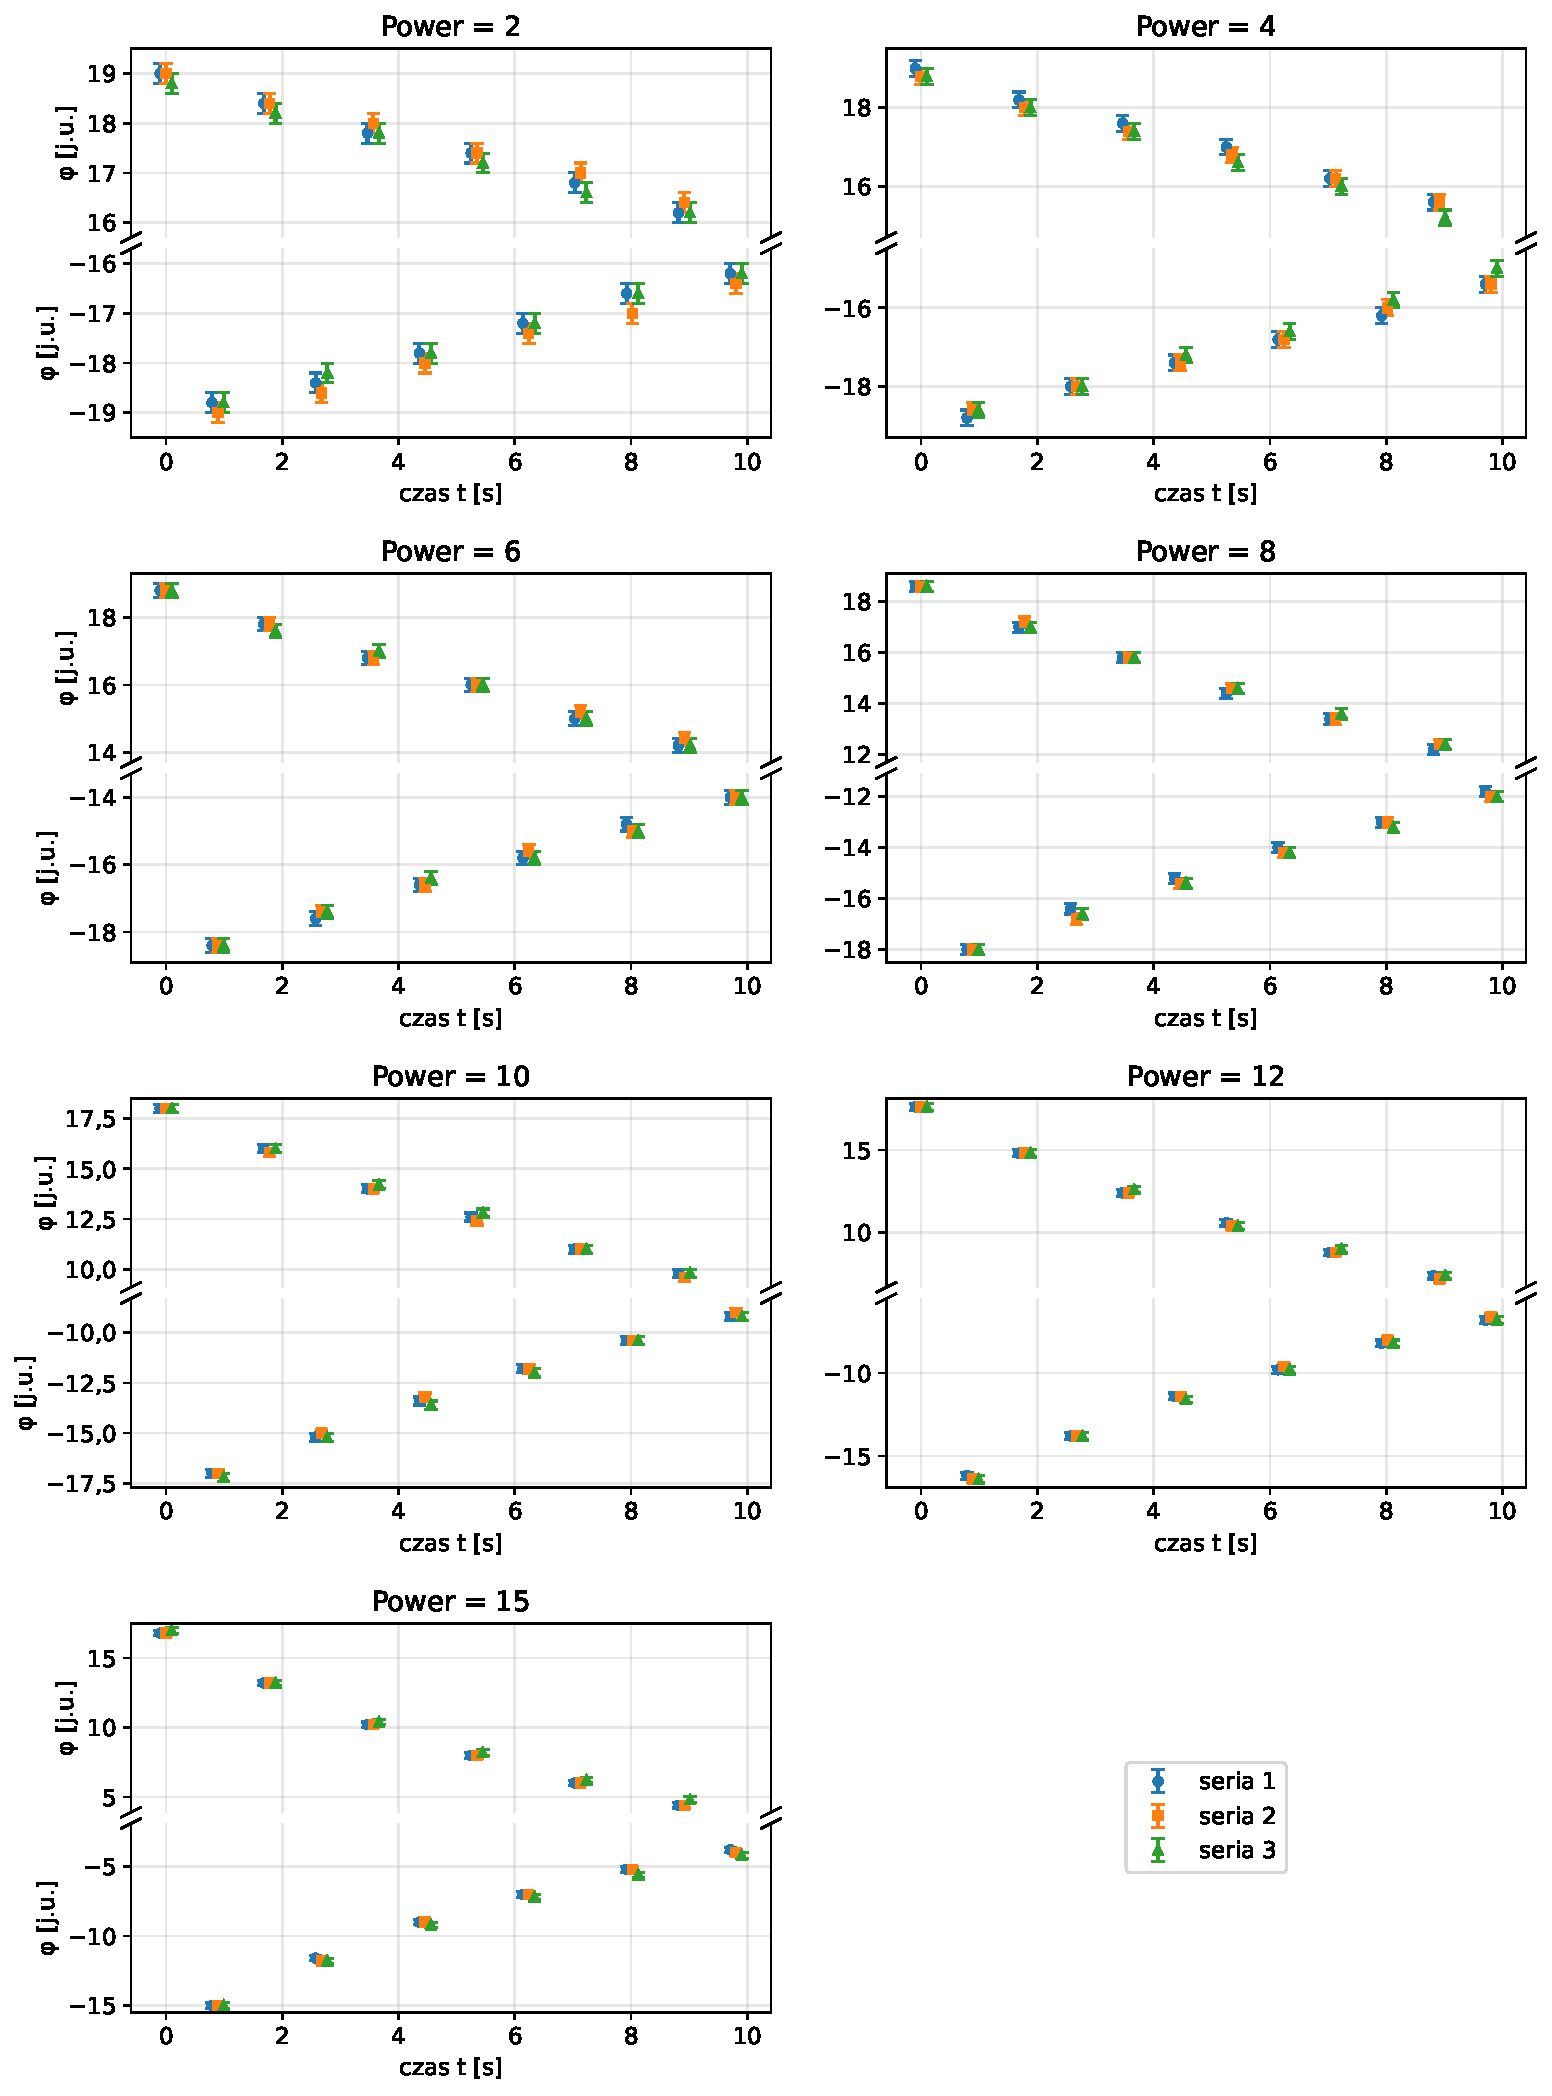
\includegraphics[width=0.9\textwidth]{damped_amplitudes_raw.pdf}
    \caption{Kolejne skrajne wychylenia wahadła $\varphi_m$ w~funkcji czasu
             $t_m = (m-1)\,T/2$ dla siedmiu nastaw hamulca. Oś pionowa jest przerwana:
             górny panel każdej nastawy pokazuje wychylenia dodatnie, dolny --- ujemne,
             oba w~tej samej skali. Różne znaczniki odpowiadają trzem seriom,
             rozsuniętym w~poziomie o~\SI{0.1}{\second} dla czytelności. Słupki błędów
             odpowiadają niepewności $u_A = 0{,}2$~j.u.}\label{fig:decay_raw}
\end{figure}

\begin{figure}[H]
    \centering
    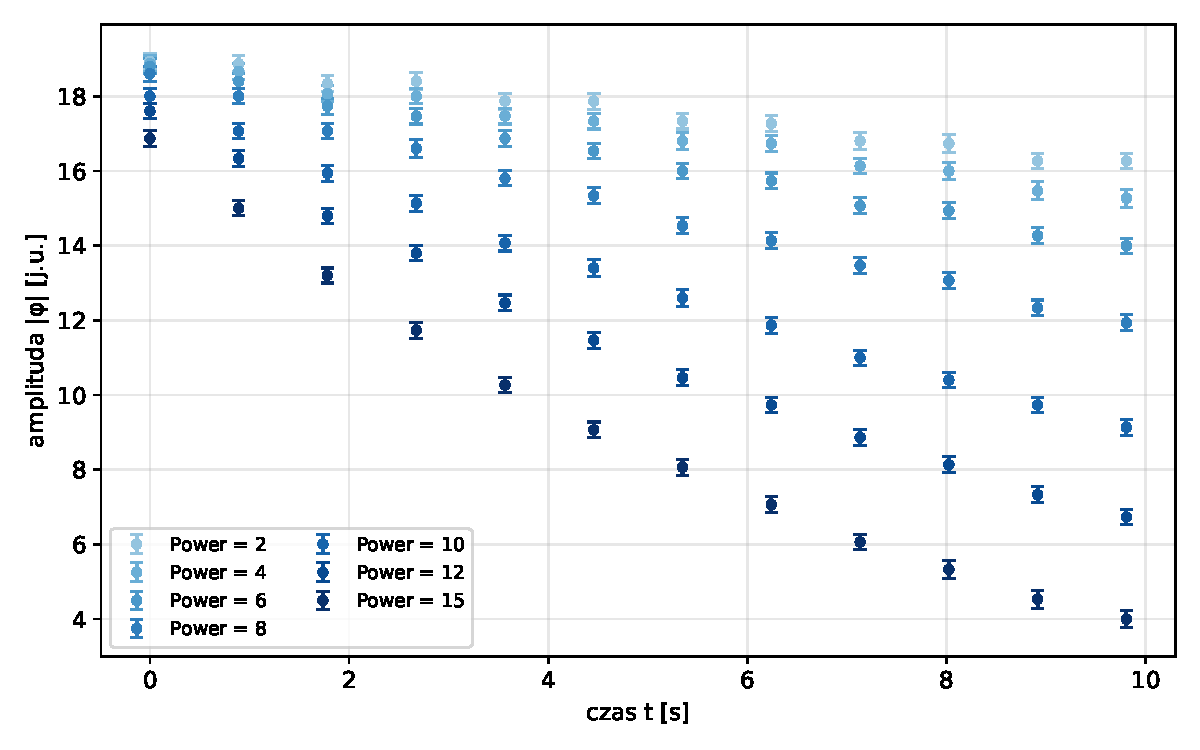
\includegraphics[width=0.82\textwidth]{damped_envelope_raw.pdf}
    \caption{Moduł skrajnych wychyleń $|\varphi_m|$ uśredniony po trzech seriach
             w~funkcji czasu dla wszystkich nastaw hamulca; ciemniejszy kolor odpowiada
             silniejszemu tłumieniu. Słupki błędów odpowiadają niepewności złożonej
             z~rozrzutu trzech serii i~$u_A$.}\label{fig:envelope_raw}
\end{figure}

\subsection{Krzywa rezonansowa}\label{sec:res_resonance}

Skrajne wychylenia wahadła w~maksimum dudnień dla kolejnych napięć zasilania
silnika zestawiono w~Tabeli~\ref{tab:resonance_raw}. Na Rysunku~\ref{fig:resonance_raw}
przedstawiono amplitudę drgań wymuszonych liczoną jako połowa rozpiętości wychyleń,
$\varphi_0 = (\varphi_+ - \varphi_-)/2$, co usuwa wpływ przesunięcia zera skali.

\begin{table}[H]
    \centering
    \caption{Skrajne wychylenia wahadła $\varphi_-$ i~$\varphi_+$ w~maksimum dudnień
             w~funkcji napięcia zasilania silnika $U$, nastawa hamulca Power~$=6$.
             Niepewności: $u_U = \SI{0.1}{\volt}$, $u_A = 0{,}6$~j.u.}\label{tab:resonance_raw}
    \begin{tabular}{S[table-format=2.2] S[table-format=-2.1] S[table-format=2.1]}
        \toprule
        {$U$ [V]} & {$\varphi_-$ [j.u.]} & {$\varphi_+$ [j.u.]} \\
        \midrule
        3.85 & -0.4 & 1.2 \\
        7.11 & -2.8 & 3.8 \\
        7.47 & -6.6 & 7.6 \\
        7.93 & -18.0 & 19.0 \\
        8.34 & -13.0 & 13.8 \\
        8.80 & -3.4 & 4.6 \\
        10.39 & -1.0 & 2.0 \\
        13.51 & 0.0 & 1.0 \\
        \bottomrule
    \end{tabular}
\end{table}

\begin{figure}[H]
    \centering
    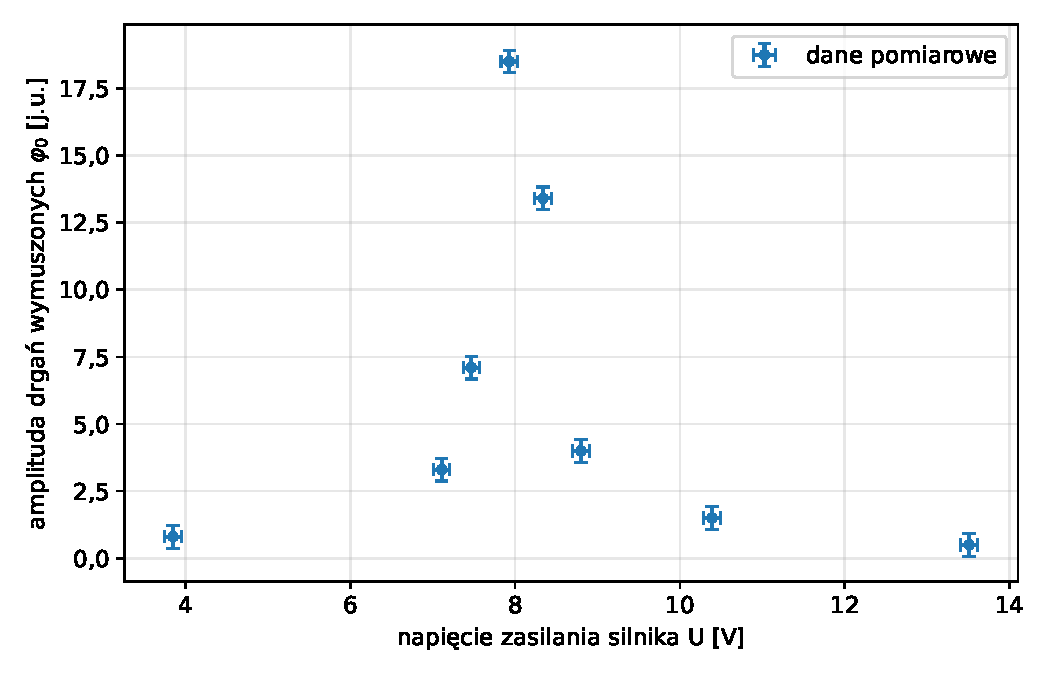
\includegraphics[width=0.82\textwidth]{resonance_curve_raw.pdf}
    \caption{Amplituda drgań wymuszonych $\varphi_0$ w~funkcji napięcia zasilania
             silnika $U$ dla nastawy hamulca Power~$=6$. Słupki błędów odpowiadają
             niepewnościom $u_U = \SI{0.1}{\volt}$
             i~$u(\varphi_0) = u_A/\sqrt{2} \approx 0{,}42$~j.u.}\label{fig:resonance_raw}
\end{figure}



% -------------------------------------------
\section{Opracowanie wyników}
% -------------------------------------------

Wszystkie dopasowania wykonano metodą najmniejszych kwadratów z~wagami
$w_i = 1/\sigma_i^2$ (funkcja \texttt{scipy.optimize.curve\_fit} z~opcją
\texttt{absolute\_sigma=True}). Niepewności parametrów to pierwiastki z~elementów
diagonalnych macierzy kowariancji, $u_{a_i} = \sqrt{C_{ii}}$. Jakość dopasowania
oceniano zredukowanym $\chi^2/\nu$, gdzie $\nu$ --- liczba punktów pomniejszona
o~liczbę parametrów. Niepewności wielkości złożonych wyznaczono z~prawa propagacji
niepewności:
\begin{equation}
    u(f) = \sqrt{\sum_i \left(\frac{\partial f}{\partial x_i}\right)^2 u^2(x_i)},
    \label{eq:propagation}
\end{equation}
a~tam, gdzie parametry dopasowania są skorelowane --- z~pełną macierzą kowariancji.

\paragraph{Niepewność pomiaru czasu.}
Jako niepewność pojedynczego pomiaru czasu stoperem przyjęto czas reakcji człowieka,
$u_T = \SI{0.3}{\second}$ (oszacowanie typu B). Przy uśrednianiu $k$~pomiarów niepewność
ta jest dzielona przez $\sqrt{k}$ --- tak samo w~średnich z~trzech pomiarów
i~w~dopasowaniu stałej do dziesięciu pomiarów $T_0$. Takie traktowanie wynika z~tego,
jak powstaje błąd reakcji. Mierzony czas to różnica chwil zatrzymania i~uruchomienia
stopera, więc stała część opóźnienia reakcji (jednakowa przy starcie i~stopie) znosi
się w~każdym pomiarze. Pozostaje różnica opóźnień przy starcie i~stopie, która jest inna
w~każdym pomiarze i~niezależna od pozostałych --- czyli ma charakter losowy i~maleje przy
uśrednianiu. Ewentualnej systematycznej różnicy między reakcją na start i~na stop nie
da się oszacować z~danych i~jej nie uwzględniono.

Nie zastąpiono $u_T$ niepewnością typu A z~rozrzutu, bo większość punktów zmierzono
tylko $k = 3$ razy. Odchylenie standardowe z~trzech pomiarów ma względną niepewność
$1/\sqrt{2(k-1)} = 50\,\%$, a~w~tym ćwiczeniu zmienia się między punktami od
\SI{0.031}{\second} do \SI{0.248}{\second}, czyli 8-krotnie. Wagi oparte na takim
rozrzucie byłyby przypadkowe: punkty, w~których trzy pomiary akurat wypadły blisko
siebie, dominowałyby w~dopasowaniach. Jednakowa dla wszystkich pomiarów wartość $u_T$
daje wagi zależne tylko od liczby mierzonych okresów i~długości mierzonego czasu.
Ceną jest zachowawczość: rozrzut dziesięciu pomiarów $5T_0$ (\SI{0.075}{\second})
jest 4~razy mniejszy od $u_T$, co widać w~wartościach $\chi^2/\nu < 1$
(Sekcje~\ref{sec:op_calibration} i~\ref{sec:op_free}). Wpływ tego wyboru na
najważniejszy wniosek oszacowano w~Sekcji~\ref{sec:op_resonance}: przy niepewności
czasu równej rozrzutowi pomiarów $5T_0$ różnica $\omega_0$ z~rezonansu i~ze stopera
rośnie z~$2{,}7\sigma$ do $4{,}5\sigma$.

Okres wyznaczony z~$k = 3$ pomiarów czasu $n$~okresów i~jego niepewność wynoszą
\begin{equation}
    T = \frac{\overline{t}}{n}, \qquad
    u(T) = \frac{u_T}{n\sqrt{k}},
    \label{eq:period}
\end{equation}
gdzie $\overline{t}$ --- średnia z~pomiarów czasu. Częstość kołowa
$\omega = 2\pi/T$ ma niepewność $u(\omega) = 2\pi\,u(T)/T^2$.

\subsection{Kalibracja częstości siły wymuszającej}\label{sec:op_calibration}

Do zależności $\Omega(U)$ dopasowano prostą
\begin{equation}
    \Omega = a\,U + b,
    \label{eq:calibration}
\end{equation}
gdzie $a$ --- współczynnik kalibracji, $b$ --- wyraz wolny. Niepewność napięcia
uwzględniono metodą wariancji efektywnej, iteracyjnie przyjmując
$\sigma_i^2 = u^2(\Omega_i) + a^2 u_U^2$. Dopasowanie przedstawiono na
Rysunku~\ref{fig:calibration_fit}. Otrzymano
\begin{equation*}
    a = \SI{0.4890 \pm 0.0056}{\radian\per\second\per\volt}, \qquad
    b = \SI{-0.256 \pm 0.037}{\radian\per\second},
\end{equation*}
przy $\mathrm{cov}(a,b) = \SI{-1.72e-4}{\radian\squared\per\second\squared\per\volt}$
i~$\chi^2/\nu = 0{,}46$.

\begin{figure}[H]
    \centering
    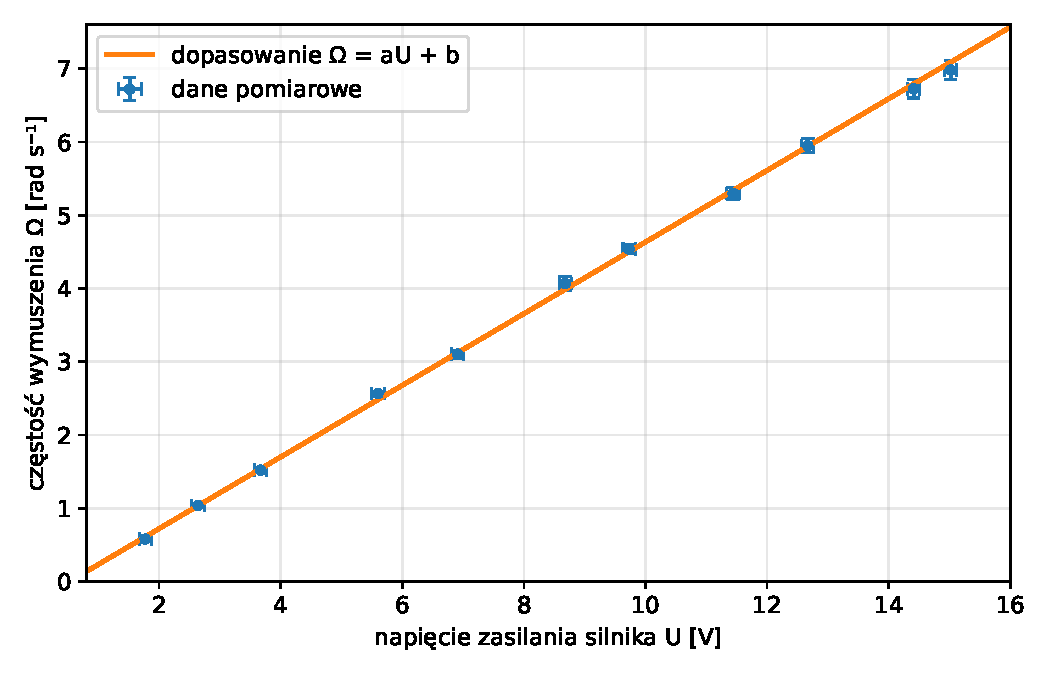
\includegraphics[width=0.72\textwidth]{force_calibration.pdf}
    \caption{Częstość siły wymuszającej $\Omega$ w~funkcji napięcia zasilania
             silnika $U$ z~dopasowaną prostą~\eqref{eq:calibration}. Słupki błędów
             odpowiadają niepewnościom $u_U$ i~$u(\Omega)$.}\label{fig:calibration_fit}
\end{figure}

Udział obu składników niepewności zależy od napięcia. Przy $U = \SI{1.77}{\volt}$
niepewność z~pomiaru czasu wynosi $u(\Omega) = \SI{0.0019}{\radian\per\second}$,
a~składnik napięciowy $a\,u_U = \SI{0.049}{\radian\per\second}$ jest 25~razy większy.
Przy $U = \SI{15.02}{\volt}$ jest odwrotnie: $u(\Omega) = \SI{0.134}{\radian\per\second}$.
Wartość $\chi^2/\nu < 1$ wskazuje więc, że zachowawcze mogą być obie przyjęte
niepewności, $u_T$ i~$u_U$.

Częstość odczytana z~prostej kalibracyjnej dla napięcia $U$ ma niepewność
\begin{equation}
    u_\text{kal}(\Omega) = \sqrt{U^2 u_a^2 + u_b^2 + 2U\,\mathrm{cov}(a,b)},
    \label{eq:u_cal}
\end{equation}
która w~okolicy rezonansu ($U \approx \SI{8}{\volt}$) wynosi
$\approx\SI{0.025}{\radian\per\second}$.

\subsection{Drgania swobodne}\label{sec:op_free}

Do dziesięciu okresów $T_0$ dopasowano stałą (Rysunek~\ref{fig:free_fit}),
co jest równoważne średniej ważonej. Otrzymano
\begin{equation*}
    T_0 = \SI{1.774 \pm 0.019}{\second}, \qquad \chi^2/\nu = 0{,}062.
\end{equation*}
Częstość drgań własnych z~wzoru~\eqref{eq:omega0} i~jej niepewność
$u(\omega_0) = 2\pi\,u(T_0)/T_0^2$ wynoszą
\begin{equation*}
    \omega_0 = \SI{3.543 \pm 0.038}{\radian\per\second}.
\end{equation*}
Odchylenie standardowe dziesięciu pomiarów, $\sigma(T_0) = \SI{0.015}{\second}$
(czyli \SI{0.075}{\second} dla pojedynczego pomiaru $5T_0$), jest 4~razy mniejsze
od niepewności pojedynczego pomiaru $u_T/5 = \SI{0.060}{\second}$. Stąd mała wartość
$\chi^2/\nu$: przyjęta niepewność czasu reakcji jest
zawyżona względem faktycznej powtarzalności pomiarów.

\begin{figure}[H]
    \centering
    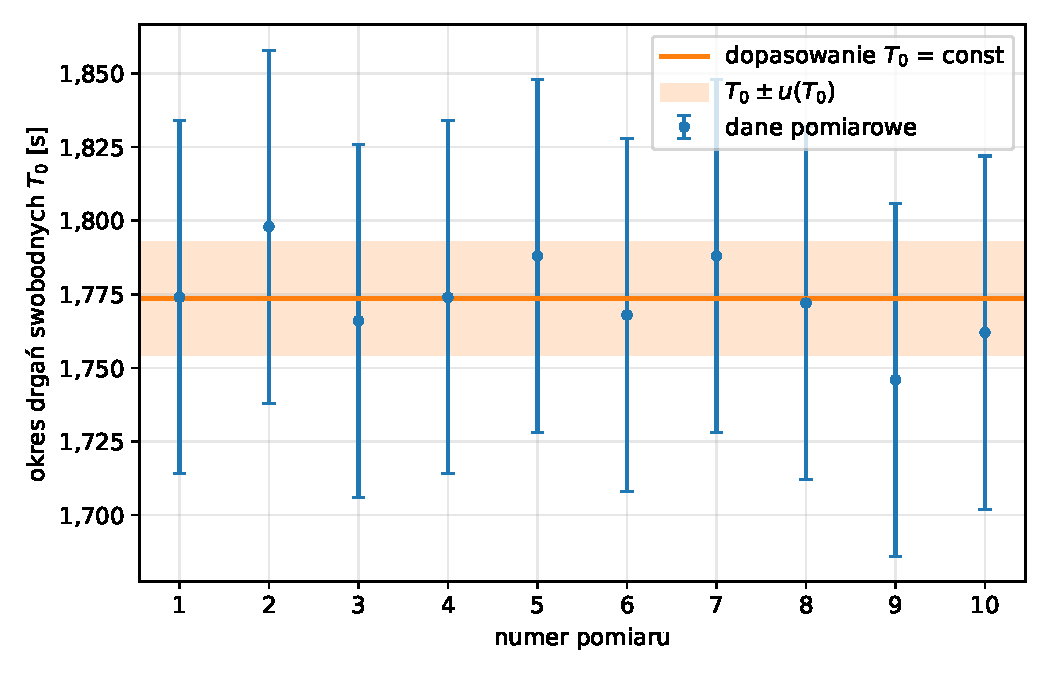
\includegraphics[width=0.72\textwidth]{free_oscillations.pdf}
    \caption{Okres drgań swobodnych $T_0$ w~kolejnych pomiarach z~dopasowaną stałą;
             pasmo odpowiada $T_0 \pm u(T_0)$. Słupki błędów odpowiadają
             niepewności $u_T/5 = \SI{0.06}{\second}$.}\label{fig:free_fit}
\end{figure}

\subsection{Okresy drgań tłumionych}\label{sec:op_damped_periods}

Okresy $T$ i~częstości $\omega$ drgań tłumionych dla kolejnych nastaw zestawiono
w~Tabeli~\ref{tab:damped_periods}. Porównano je z~częstością przewidywaną przez
wzór~\eqref{eq:omega_damped}, $\omega_\text{teor} = \sqrt{\omega_0^2 - (\Gamma/2)^2}$,
z~$\omega_0$ z~Sekcji~\ref{sec:op_free} i~$\Gamma$ z~zaniku amplitudy
(Sekcja~\ref{sec:op_decay}). Niepewność:
\begin{equation}
    u(\omega_\text{teor}) = \sqrt{\left(\frac{\omega_0}{\omega_\text{teor}}\,u(\omega_0)\right)^2
                          + \left(\frac{\Gamma}{4\omega_\text{teor}}\,u(\Gamma)\right)^2}.
    \label{eq:u_omega_teor}
\end{equation}

\begin{table}[H]
    \centering
    \caption{Okresy $T$ i~częstości $\omega$ drgań tłumionych, częstość teoretyczna
             $\omega_\text{teor}$ z~wzoru~\eqref{eq:omega_damped}, przewidywane
             przesunięcie $\Delta\omega_\text{teor} = \omega_0 - \omega_\text{teor}$
             oraz odległość $|T - T_0|/\sqrt{u^2(T) + u^2(T_0)}$.}\label{tab:damped_periods}
    \begin{tabular}{S[table-format=2.0]
                    S[table-format=1.3]@{\,$\pm$\,}S[table-format=1.3]
                    S[table-format=1.3]@{\,$\pm$\,}S[table-format=1.3]
                    S[table-format=1.3]@{\,$\pm$\,}S[table-format=1.3]
                    S[table-format=1.2] S[table-format=1.2]}
        \toprule
        {Power} & \multicolumn{2}{c}{$T$ [\si{\second}]}
        & \multicolumn{2}{c}{$\omega$ [\si{\radian\per\second}]}
        & \multicolumn{2}{c}{$\omega_\text{teor}$ [\si{\radian\per\second}]}
        & {$\Delta\omega_\text{teor}$ [\si{\milli\radian\per\second}]} & {$|T-T_0|/u$} \\
        \midrule
        2 & 1.774 & 0.035 & 3.542 & 0.069 & 3.543 & 0.038 & 0.04 & 0.01 \\
        4 & 1.780 & 0.035 & 3.530 & 0.069 & 3.543 & 0.038 & 0.07 & 0.16 \\
        6 & 1.787 & 0.035 & 3.517 & 0.068 & 3.542 & 0.038 & 0.13 & 0.33 \\
        8 & 1.797 & 0.035 & 3.496 & 0.067 & 3.542 & 0.038 & 0.29 & 0.60 \\
        10 & 1.791 & 0.035 & 3.509 & 0.068 & 3.542 & 0.038 & 0.67 & 0.43 \\
        12 & 1.784 & 0.035 & 3.522 & 0.068 & 3.541 & 0.038 & 1.35 & 0.26 \\
        15 & 1.767 & 0.035 & 3.555 & 0.070 & 3.540 & 0.038 & 2.91 & 0.16 \\
        \bottomrule
    \end{tabular}
\end{table}

Wszystkie okresy tłumione są zgodne z~$T_0$ (odległość $\leq 0{,}6\sigma$).
Dopasowanie stałej do wszystkich siedmiu okresów daje
$T = \SI{1.783 \pm 0.013}{\second}$ przy $\chi^2/\nu = 0{,}085$, zgodne z~$T_0$
($0{,}4\sigma$). Największe przewidywane przesunięcie częstości, dla Power~$=15$,
wynosi $\Delta\omega_\text{teor} = \SI{2.9e-3}{\radian\per\second}$, co odpowiada
wydłużeniu okresu o~\SI{1.5}{\milli\second}. Stanowi to $4{,}2\,\%$ niepewności
$u(\omega) = \SI{0.070}{\radian\per\second}$, więc wpływ tłumienia na okres jest
niemierzalny tą metodą. Pokazuje to Rysunek~\ref{fig:damped_periods_fit}.

\begin{figure}[H]
    \centering
    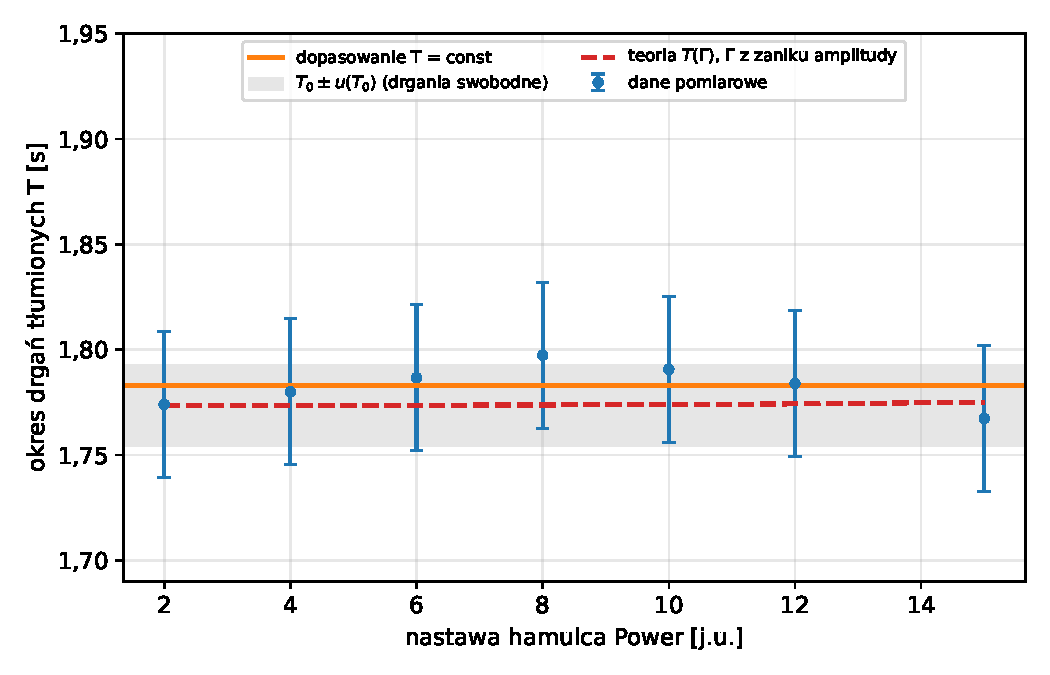
\includegraphics[width=0.72\textwidth]{damped_periods.pdf}
    \caption{Okres drgań tłumionych $T$ w~funkcji nastawy hamulca z~dopasowaną
             stałą (linia pomarańczowa), pasmem $T_0 \pm u(T_0)$ z~drgań swobodnych
             (szare) i~przewidywaniem $T(\Gamma)$ z~wzoru~\eqref{eq:omega_damped}
             (linia przerywana). Słupki błędów odpowiadają niepewności $u(T)$.}
    \label{fig:damped_periods_fit}
\end{figure}

\subsection{Zanik amplitudy drgań tłumionych}\label{sec:op_decay}

Dla każdej nastawy hamulca do wszystkich $3 \times 12 = 36$ wychyleń dopasowano
jednocześnie model wynikający ze wzoru~\eqref{eq:extrema}, uzupełniony o~przesunięcie
zera skali:
\begin{equation}
    \varphi_m = (-1)^{m-1} A\,e^{-\Gamma t_m/2} + c, \qquad t_m = (m-1)\,\frac{T}{2},
    \label{eq:decay_model}
\end{equation}
gdzie $A$ --- amplituda pierwszego odczytanego ekstremum, $\Gamma$ --- parametr
tłumienia, $c$ --- przesunięcie zera skali względem położenia równowagi,
$T$ --- okres drgań tłumionych, a~czas $t_m$ liczony jest od pierwszego odczytanego
ekstremum. Każdy punkt ma niepewność $u_A = 0{,}2$~j.u.
Parametry dopasowania zestawiono w~Tabeli~\ref{tab:decay_fit}, a~dopasowane obwiednie
przedstawiono na Rysunkach~\ref{fig:decay_fit} i~\ref{fig:envelope_fit}.

Okres $T$ jest w~modelu~\eqref{eq:decay_model} ustalony, a~nie dopasowywany: dane
zawierają tylko wartości kolejnych ekstremów, bez chwil ich wystąpienia, więc z~samego
zaniku wyznacza się jedynie iloczyn $\Gamma T$. Dla wszystkich nastaw przyjęto wspólny
okres $T = \SI{1.783 \pm 0.013}{\second}$ z~Sekcji~\ref{sec:op_damped_periods}:
wszystkie okresy tłumione są ze sobą zgodne, a~teoretyczna zależność okresu od $\Gamma$
nie przekracza $0{,}1\,\%$. Osobne okresy dla każdej nastawy wnosiłyby do $\Gamma$
niepotrzebny losowy rozrzut rzędu $2\,\%$. Ponieważ wyznaczany jest iloczyn $\Gamma T$,
niepewność okresu przenosi się na parametr tłumienia:
\begin{equation}
    \frac{u(\Gamma)}{\Gamma} = \sqrt{\left(\frac{u_\text{fit}(\Gamma)}{\Gamma}\right)^2
                             + \left(\frac{u(T)}{T}\right)^2},
    \label{eq:u_Gamma}
\end{equation}
gdzie $u_\text{fit}(\Gamma)$ --- niepewność z~dopasowania, a~$u(T)/T = 0{,}73\,\%$ jest
wspólnym czynnikiem skali dla wszystkich nastaw.

\begin{table}[H]
    \centering
    \caption{Parametry dopasowania modelu~\eqref{eq:decay_model} do zaniku
             amplitudy dla kolejnych nastaw hamulca. Niepewność $\Gamma$ zawiera
             niepewność okresu (wzór~\eqref{eq:u_Gamma}).}\label{tab:decay_fit}
    \begin{tabular}{S[table-format=2.0]
                    S[table-format=2.3]@{\,$\pm$\,}S[table-format=1.3]
                    S[table-format=1.4]@{\,$\pm$\,}S[table-format=1.4]
                    S[table-format=-1.3]@{\,$\pm$\,}S[table-format=1.3]
                    S[table-format=1.2]}
        \toprule
        {Power} & \multicolumn{2}{c}{$A$ [j.u.]}
        & \multicolumn{2}{c}{$\Gamma$ [\si{\per\second}]}
        & \multicolumn{2}{c}{$c$ [j.u.]} & {$\chi^2/\nu$} \\
        \midrule
        2 & 19.069 & 0.065 & 0.0338 & 0.0013 & -0.121 & 0.034 & 0.42 \\
        4 & 18.974 & 0.066 & 0.0441 & 0.0013 & -0.101 & 0.034 & 0.50 \\
        6 & 18.860 & 0.067 & 0.0609 & 0.0014 & -0.082 & 0.034 & 0.22 \\
        8 & 18.665 & 0.069 & 0.0912 & 0.0016 & -0.079 & 0.034 & 0.26 \\
        10 & 18.101 & 0.072 & 0.1381 & 0.0020 & -0.045 & 0.034 & 0.36 \\
        12 & 17.724 & 0.076 & 0.1955 & 0.0025 & -0.055 & 0.034 & 0.29 \\
        15 & 17.037 & 0.081 & 0.2871 & 0.0034 & -0.026 & 0.034 & 0.73 \\
        \bottomrule
    \end{tabular}
\end{table}

\begin{figure}[H]
    \centering
    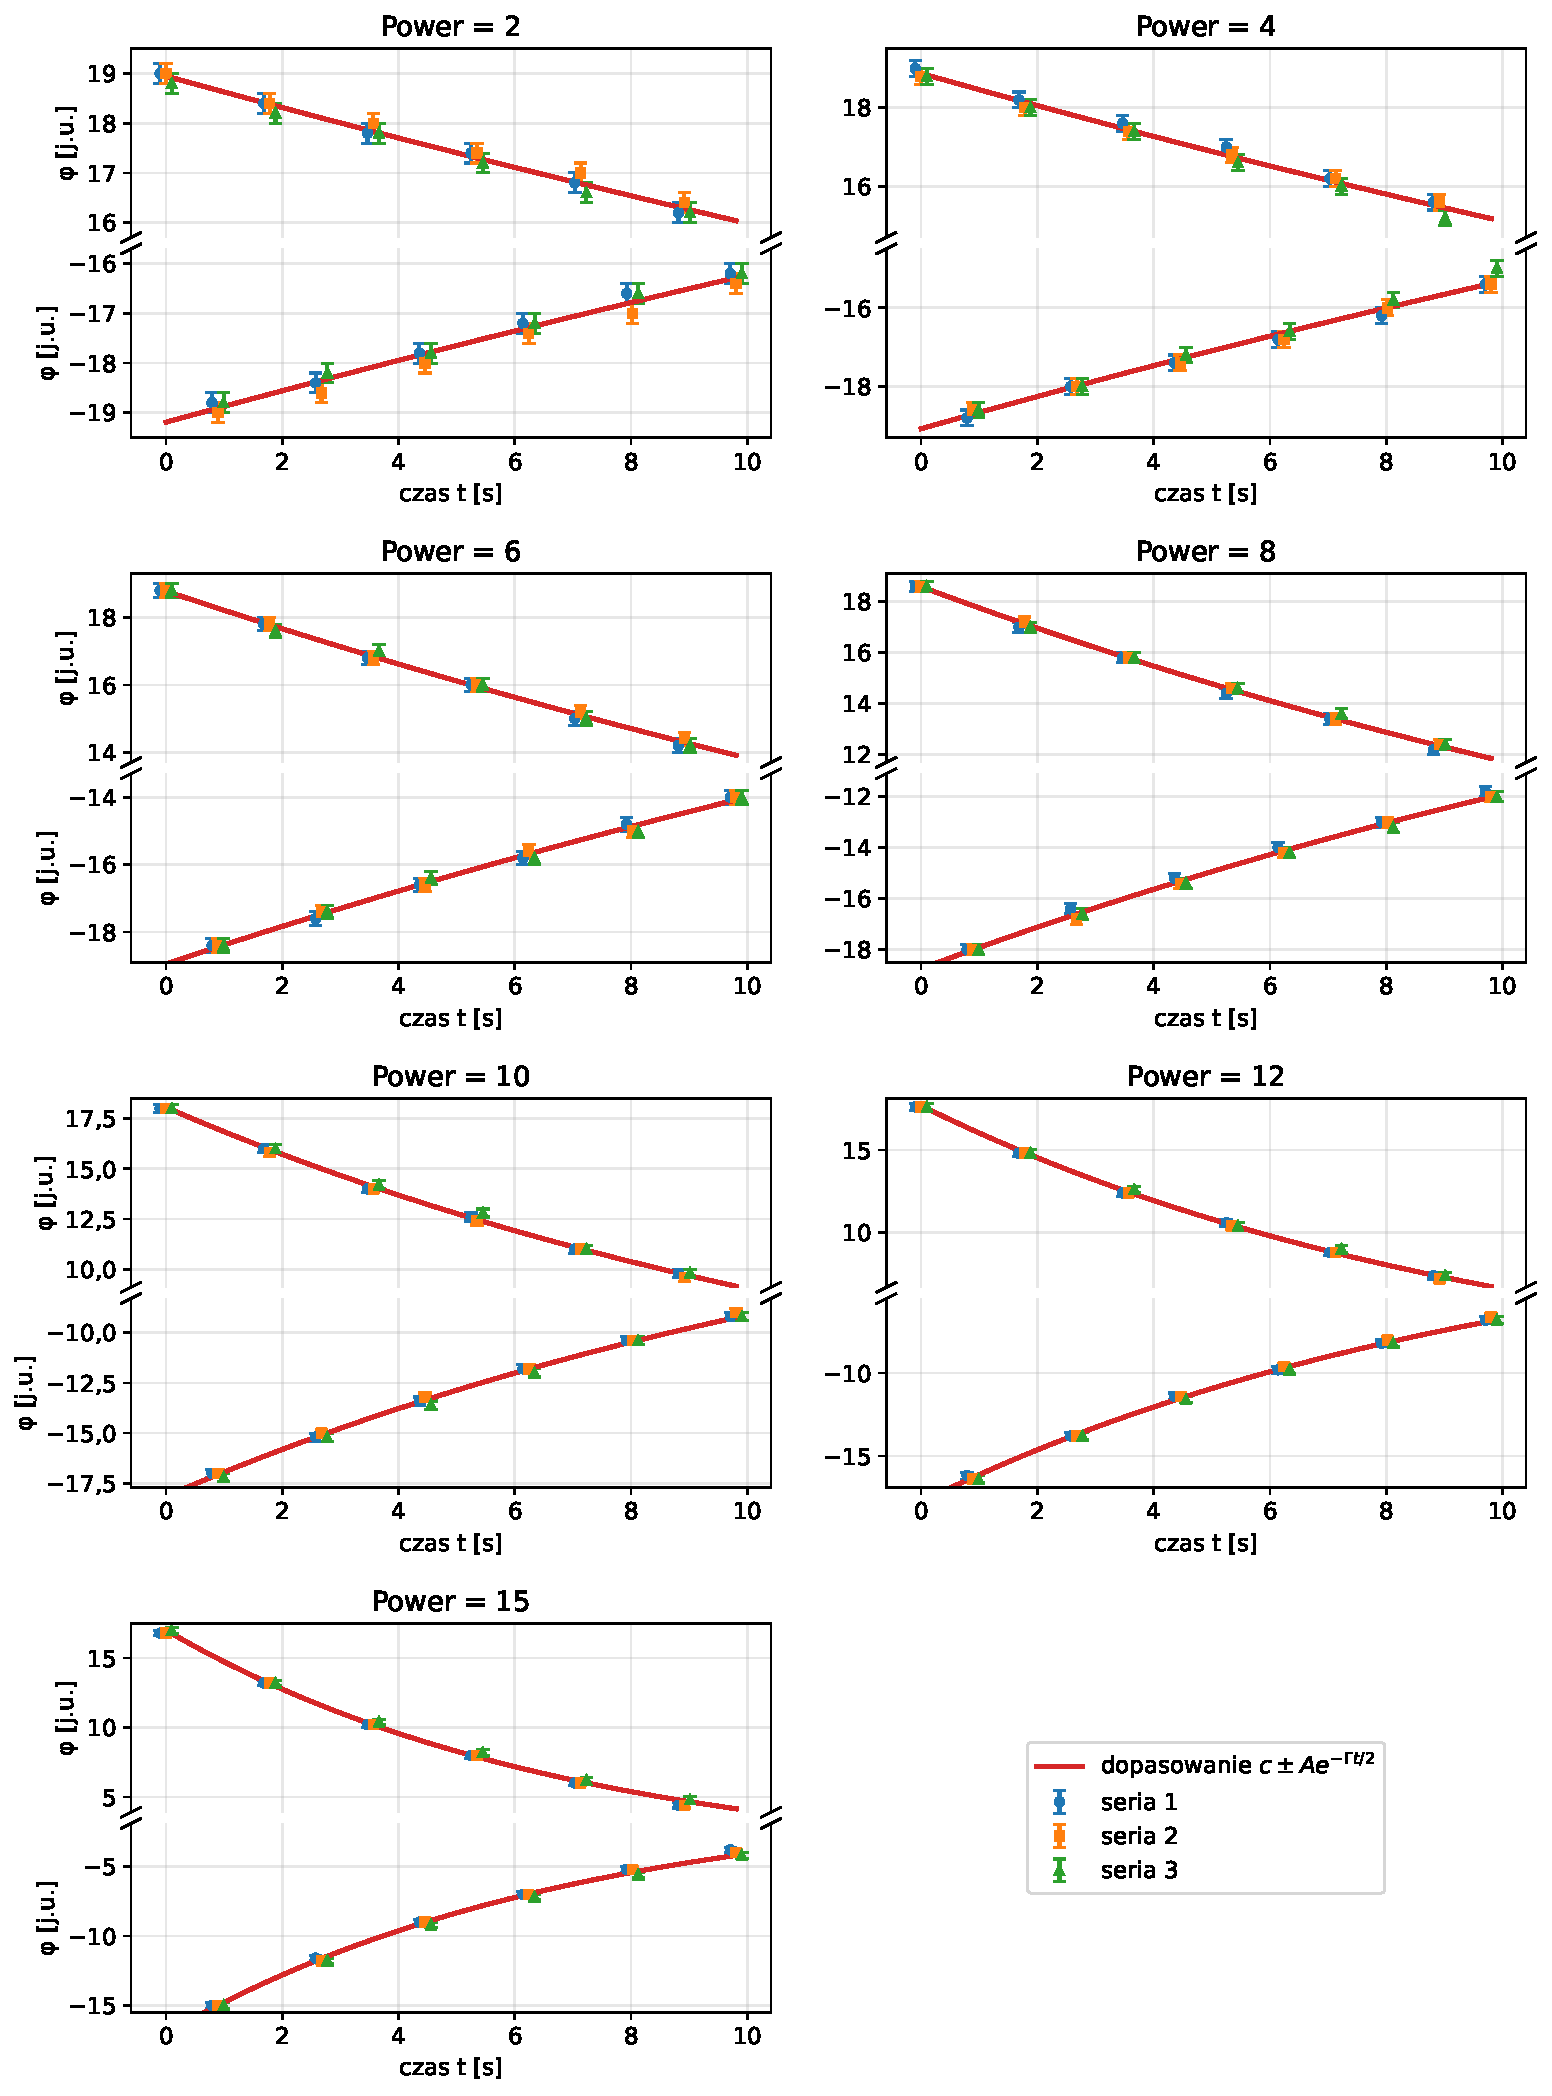
\includegraphics[width=0.9\textwidth]{damped_amplitudes.pdf}
    \caption{Kolejne skrajne wychylenia wahadła $\varphi_m$ w~funkcji czasu
             z~dopasowaną obwiednią $c \pm A e^{-\Gamma t/2}$
             (model~\eqref{eq:decay_model}). Oś pionowa przerwana jak na
             Rysunku~\ref{fig:decay_raw}. Słupki błędów odpowiadają niepewności
             $u_A = 0{,}2$~j.u.}\label{fig:decay_fit}
\end{figure}

\begin{figure}[H]
    \centering
    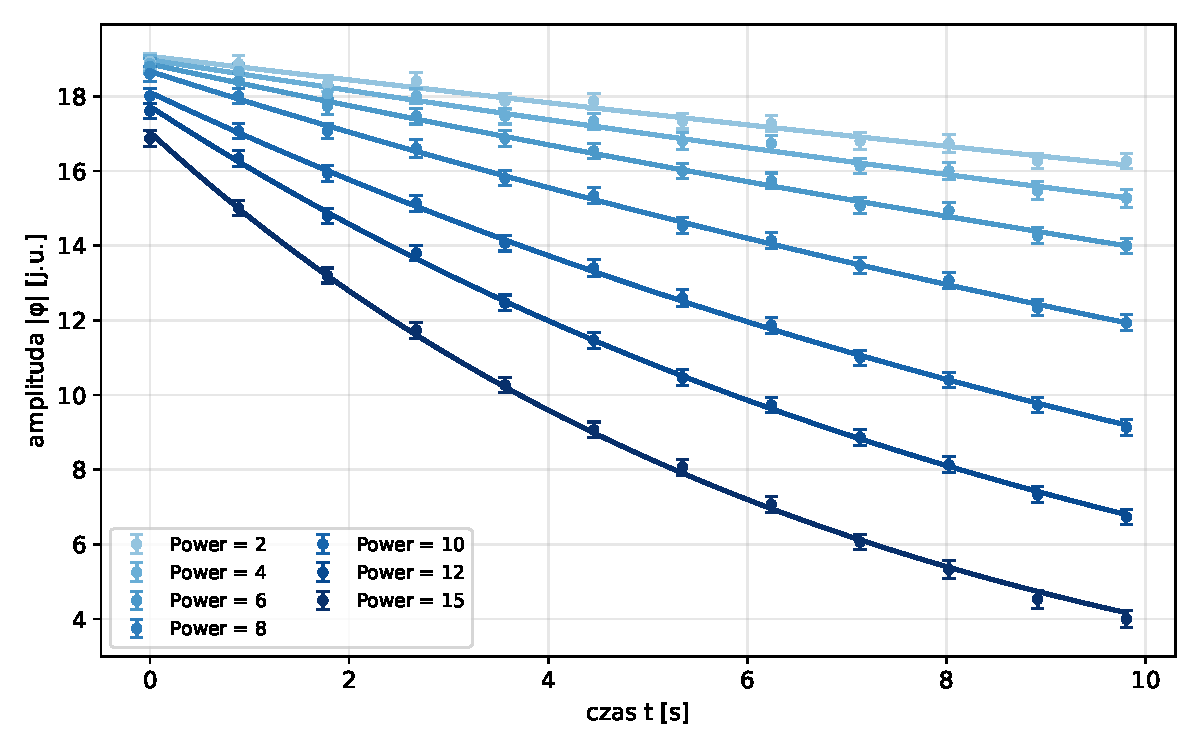
\includegraphics[width=0.82\textwidth]{damped_envelope.pdf}
    \caption{Moduł skrajnych wychyleń $|\varphi_m|$ uśredniony po trzech seriach
             z~dopasowanymi obwiedniami $A e^{-\Gamma t/2}$ dla wszystkich nastaw
             hamulca. Słupki błędów odpowiadają niepewności złożonej z~rozrzutu
             trzech serii i~$u_A$.}\label{fig:envelope_fit}
\end{figure}

Wartości $\chi^2/\nu = 0{,}22$--$0{,}73$ wskazują, że $u_A = 0{,}2$~j.u.\ jest
niepewnością zachowawczą. Parametr $A$ maleje z~nastawą hamulca (od $19{,}07$
do $17{,}04$~j.u.), choć wahadło puszczano zawsze z~tego samego, maksymalnego
wychylenia. Zgadza się to z~założeniem, że pierwsze odczytane ekstremum wystąpiło
pół okresu po puszczeniu: odpowiadające mu wychylenie startowe $A\,e^{\Gamma T/4}$
wynosi dla wszystkich siedmiu nastaw od $19{,}25$ do $19{,}44$~j.u., średnio
$19{,}35 \pm 0{,}06$~j.u. Wahadło puszczano więc z~około $19{,}4$~j.u., nieco więcej
niż największy odczytany z~nagrań wychylenie $19{,}0$~j.u. Przesunięcie początku osi
czasu nie zmienia wyznaczonego $\Gamma$.

Z~parametru tłumienia wyznaczono czas relaksacji~\eqref{eq:tau} i~dobroć~\eqref{eq:Q}
z~niepewnościami
\begin{equation}
    u(\tau) = \frac{u(\Gamma)}{\Gamma^2}, \qquad
    u(Q) = Q\sqrt{\left(\frac{u(\omega_0)}{\omega_0}\right)^2 + \left(\frac{u(\Gamma)}{\Gamma}\right)^2}.
    \label{eq:tau_Q}
\end{equation}
Wyniki zestawiono w~Tabeli~\ref{tab:decay_derived}. We wszystkich nastawach
$\Gamma/\Gamma_\text{kr} = \Gamma/(2\omega_0) \leq 4{,}05\,\%$, czyli tłumienie jest słabe.
Dla porównania w~Tabeli~\ref{tab:decay_derived} podano też $\Gamma_\text{lin}$
z~linearyzacji sugerowanej w~skrypcie~\cite{skrypt}: regresji liniowej ważonej
$\ln|\varphi_m| = \ln A - \tfrac{\Gamma}{2}\,t_m$ z~$u(\ln|\varphi_m|) = u_A/|\varphi_m|$
(niepewność $\Gamma_\text{lin}$ podano bez wspólnego czynnika od $u(T)$).
Wartości różnią się o~najwyżej $0{,}5\,u(\Gamma)$; nie jest to niezależna weryfikacja,
bo obie metody korzystają z~tych samych danych i~różnią się głównie uwzględnieniem
przesunięcia $c$. Dopasowanie modelu osobno do każdej serii daje rozrzut $\Gamma$
między seriami (odchylenie standardowe średniej) równy $0{,}4$--$1{,}2$ niepewności
$u(\Gamma)$, więc $u(\Gamma)$ dobrze opisuje powtarzalność pomiaru.

\begin{table}[H]
    \centering
    \caption{Czas relaksacji $\tau$, dobroć $Q$, stosunek $\Gamma/\Gamma_\text{kr}$
             i~parametr tłumienia z~linearyzacji $\Gamma_\text{lin}$ dla kolejnych
             nastaw hamulca.}\label{tab:decay_derived}
    \begin{tabular}{S[table-format=2.0]
                    S[table-format=2.3]@{\,$\pm$\,}S[table-format=1.3]
                    S[table-format=3.2]@{\,$\pm$\,}S[table-format=1.2]
                    S[table-format=1.2]
                    S[table-format=1.4]@{\,$\pm$\,}S[table-format=1.4]}
        \toprule
        {Power} & \multicolumn{2}{c}{$\tau$ [\si{\second}]} & \multicolumn{2}{c}{$Q$}
        & {$\Gamma/\Gamma_\text{kr}$ [\%]}
        & \multicolumn{2}{c}{$\Gamma_\text{lin}$ [\si{\per\second}]} \\
        \midrule
        2 & 29.6 & 1.1 & 104.9 & 4.1 & 0.48 & 0.0331 & 0.0012 \\
        4 & 22.65 & 0.68 & 80.2 & 2.6 & 0.62 & 0.0435 & 0.0013 \\
        6 & 16.43 & 0.38 & 58.2 & 1.5 & 0.86 & 0.0604 & 0.0013 \\
        8 & 10.96 & 0.19 & 38.83 & 0.80 & 1.29 & 0.0907 & 0.0015 \\
        10 & 7.24 & 0.10 & 25.65 & 0.46 & 1.95 & 0.1378 & 0.0017 \\
        12 & 5.115 & 0.065 & 18.12 & 0.30 & 2.76 & 0.1950 & 0.0020 \\
        15 & 3.484 & 0.041 & 12.34 & 0.20 & 4.05 & 0.2863 & 0.0027 \\
        \bottomrule
    \end{tabular}
\end{table}

\paragraph{Tłumienie lepkie a~tarcie suche.}
Model~\eqref{eq:damped} zakłada moment hamujący proporcjonalny do prędkości kątowej.
Dla tarcia suchego (stały moment hamujący) amplituda malałaby liniowo, o~stałą wartość
co pół okresu: $\varphi_m = (-1)^{m-1}(A - \kappa\,t_m) + c$. Ten model dopasowano
w~ten sam sposób; porównanie zestawiono w~Tabeli~\ref{tab:dry_friction}.
Dla Power~$\leq 6$, gdy amplituda w~czasie pomiaru maleje o~najwyżej $26\,\%$,
oba modele opisują dane równie dobrze. Dla Power~$\geq 10$ model liniowy jest
wyraźnie gorszy ($\chi^2/\nu = 12{,}4$ wobec $0{,}73$ dla Power~$=15$), a~wykładniczy
pozostaje zgodny z~danymi.

\begin{table}[H]
    \centering
    \caption{Porównanie $\chi^2/\nu$ dopasowań modelu wykładniczego~\eqref{eq:decay_model}
             (tłumienie lepkie) i~liniowego (tarcie suche) oraz względny spadek
             amplitudy w~czasie pomiaru.}\label{tab:dry_friction}
    \begin{tabular}{S[table-format=2.0] S[table-format=1.2] S[table-format=2.2] S[table-format=2.1]}
        \toprule
        {Power} & {$\chi^2/\nu$ (wykładniczy)} & {$\chi^2/\nu$ (liniowy)}
        & {spadek amplitudy [\%]} \\
        \midrule
        2 & 0.42 & 0.41 & 15.3 \\
        4 & 0.50 & 0.46 & 19.5 \\
        6 & 0.22 & 0.26 & 25.8 \\
        8 & 0.26 & 0.62 & 36.1 \\
        10 & 0.36 & 1.61 & 49.2 \\
        12 & 0.29 & 4.92 & 61.7 \\
        15 & 0.73 & 12.37 & 75.5 \\
        \bottomrule
    \end{tabular}
\end{table}

\paragraph{Przesunięcie zera skali.}
W~pomiarach zaniku przesunięcie $c$ wynosi od $-0{,}121$ do $-0{,}026$~j.u.\
(do $3{,}6\,u(c)$ dla Power~$=2$) i~słabo rośnie z~nastawą: dopasowanie prostej daje
nachylenie $0{,}0070 \pm 0{,}0030$~j.u.\ na jednostkę nastawy, czyli $2{,}3\sigma$.
W~pomiarze krzywej rezonansowej przesunięcie $(\varphi_+ + \varphi_-)/2$ wynosi stale
$0{,}4$--$0{,}6$~j.u., średnio $+0{,}49$~j.u. Prawdopodobną przyczyną jest mimośród
silnika: pręt łączący go ze sprężyną wyznacza zaczep sprężyny, więc położenie
równowagi wahadła zależy od tego, w~jakim położeniu mimośród się zatrzymał. Przy
pomiarach zaniku silnik był nieruchomy, a~przy krzywej rezonansowej obracał się.
W~obu przypadkach przesunięcie stanowi najwyżej kilka procent amplitudy, a~w~krzywej
rezonansowej jest eliminowane przez liczenie amplitudy z~rozpiętości wychyleń.

\paragraph{Zależność $\Gamma$ od nastawy hamulca.}
Siła hamowania prądami wirowymi jest proporcjonalna do kwadratu indukcji pola,
a~więc do kwadratu prądu elektromagnesu. Do zależności $\Gamma(P)$ dopasowano model
\begin{equation}
    \Gamma(P) = \Gamma_0 + k P^n,
    \label{eq:gamma_power}
\end{equation}
gdzie $P$ --- nastawa Power, $\Gamma_0$ --- tłumienie własne wahadła (tarcie
w~łożysku, opór powietrza), $k$ i~$n$ --- parametry hamulca
(Rysunek~\ref{fig:gamma_power}). Jako wag użyto tylko niepewności z~dopasowania
$u_\text{fit}(\Gamma)$: niepewność wspólnego okresu zmienia wszystkie $\Gamma$ o~ten sam
czynnik, więc nie wpływa na $\chi^2$ ani na wykładnik $n$, a~do $\Gamma_0$ dołączono ją
na końcu. Dopasowanie ma $\chi^2/\nu = 6{,}1$: reszty sięgają $3{,}1\,u_\text{fit}(\Gamma)$
i~zmieniają znak bez wyraźnego trendu, więc model nie opisuje danych w~granicach
niepewności. Nie jest to skutek pominięcia niepewności okresu --- ta przy wspólnym $T$
nie zmienia rozrzutu punktów względem modelu. Niepewności parametrów przeskalowano
o~$\sqrt{\chi^2/\nu} = 2{,}5$, otrzymując
$\Gamma_0 = \SI{0.0296 \pm 0.0029}{\per\second}$ ($\tau_0 = \SI{33.8 \pm 3.4}{\second}$)
oraz $n = 2{,}23 \pm 0{,}10$. Model z~ustalonym $n = 2$ opisuje dane jeszcze gorzej
($\chi^2/\nu = 12{,}0$). Nie mierzono prądu elektromagnesu, więc nie da się
sprawdzić, czy rozrzut wynika z~nieliniowej skali pokrętła Power, czy
z~niepowtarzalności jego ustawienia. $\Gamma_0$ pochodzi z~ekstrapolacji do $P = 0$,
bo nie mierzono zaniku amplitudy przy wyłączonym hamulcu.

\begin{figure}[H]
    \centering
    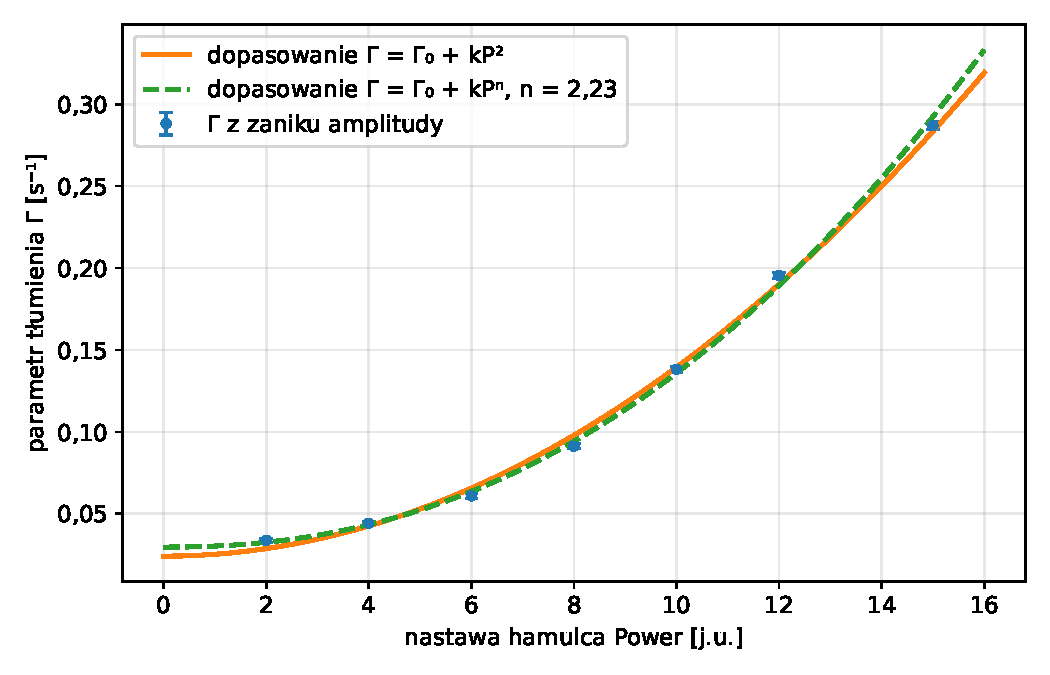
\includegraphics[width=0.72\textwidth]{gamma_vs_power.pdf}
    \caption{Parametr tłumienia $\Gamma$ w~funkcji nastawy hamulca z~dopasowanymi
             modelami $\Gamma_0 + kP^2$ (linia ciągła) i~$\Gamma_0 + kP^n$
             (linia przerywana, wzór~\eqref{eq:gamma_power}). Słupki błędów
             odpowiadają niepewności z~dopasowania $u_\text{fit}(\Gamma)$, bez wspólnego
             czynnika od niepewności okresu.}
    \label{fig:gamma_power}
\end{figure}

\subsection{Krzywa rezonansowa}\label{sec:op_resonance}

Amplitudę drgań wymuszonych wyznaczono jako połowę rozpiętości wychyleń
\begin{equation}
    \varphi_0 = \frac{\varphi_+ - \varphi_-}{2}, \qquad
    u(\varphi_0) = \frac{u_A}{\sqrt{2}} \approx 0{,}42~\text{j.u.},
    \label{eq:phi0}
\end{equation}
co usuwa przesunięcie zera skali. Napięcia przeliczono na częstość z~prostej
kalibracyjnej~\eqref{eq:calibration} i~dopasowano model~\eqref{eq:resonance}
z~parametrami $f_0$, $\omega_0$ i~$\Gamma$ (Rysunek~\ref{fig:resonance_fit}).
Niepewność częstości, $a\,u_U = \SI{0.049}{\radian\per\second}$, uwzględniono metodą
wariancji efektywnej: $\sigma_i^2 = u^2(\varphi_{0,i}) +
(\partial\varphi_0/\partial\Omega)^2\,a^2 u_U^2$, iteracyjnie. Na stromych zboczach
krzywej daje to $\sigma_i$ od $0{,}42$ do $4{,}1$~j.u., a~dla punktu w~maksimum
(\SI{7.93}{\volt}) aż $14{,}6$~j.u.

Częstość rezonansową obliczono z~wzoru~\eqref{eq:omega_r}, a~jej niepewność z~pełną
macierzą kowariancji parametrów $\omega_0$ i~$\Gamma$. Do niepewności $\omega_0$
i~$\omega_r$ z~dopasowania dodano niepewność kalibracji
$u_\text{kal} = \SI{0.025}{\radian\per\second}$ (wzór~\eqref{eq:u_cal} dla
$U \approx \SI{8.1}{\volt}$), ponieważ błąd prostej kalibracyjnej przesuwa całą krzywą
wzdłuż osi $\Omega$. Otrzymano:
\begin{gather*}
    f_0 = (12{,}1 \pm 1{,}1)~\text{j.u.}\cdot\si{\radian\squared\per\second\squared}, \qquad
    \Gamma = \SI{0.06 \pm 0.22}{\per\second}, \\
    \omega_0 = \SI{3.686 \pm 0.036}{\radian\per\second}, \qquad
    \omega_r = \SI{3.686 \pm 0.036}{\radian\per\second},
\end{gather*}
przy $\chi^2/\nu = 0{,}69$. Niepewność kalibracji odpowiada za $49\,\%$ wariancji
$u^2(\omega_0)$. Parametr tłumienia nie jest wyznaczony: $u(\Gamma)$ jest prawie
4~razy większa od samej wartości. Dopasowanie z~pominięciem niepewności napięcia
daje $\chi^2/\nu = 2{,}85$, $\omega_0 = \SI{3.702 \pm 0.025}{\radian\per\second}$
i~pozornie dobrze określone $\Gamma = \SI{0.113 \pm 0.025}{\per\second}$; wysokie
$\chi^2/\nu$ wynika tam z~pominięcia składnika $a\,u_U$, który na zboczach dominuje.

\begin{figure}[H]
    \centering
    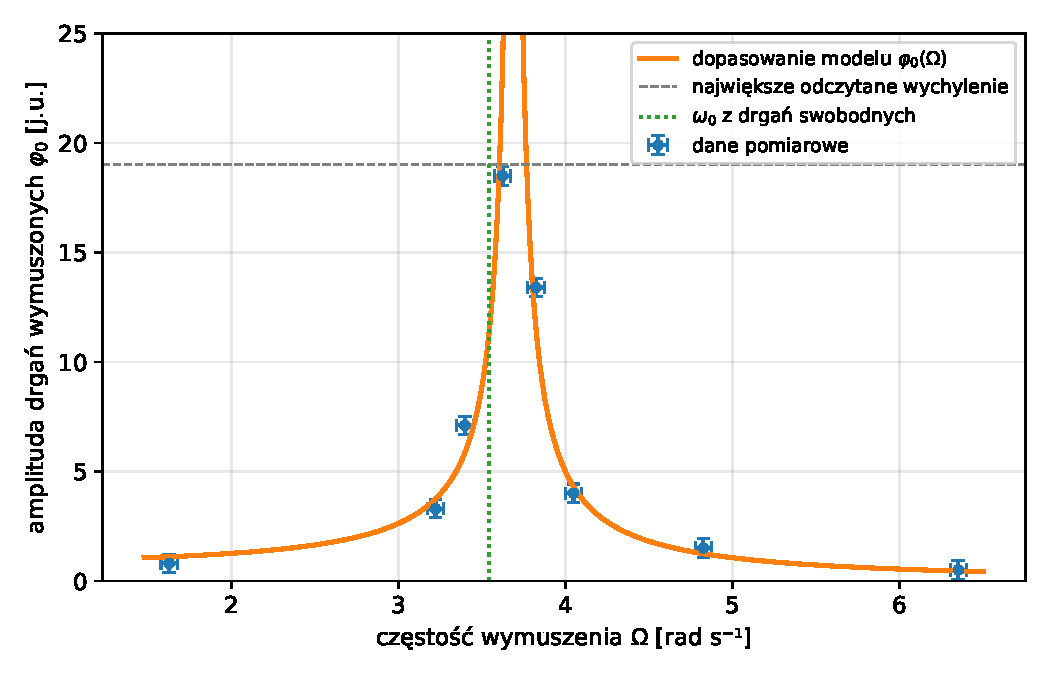
\includegraphics[width=0.72\textwidth]{resonance_curve.pdf}
    \caption{Amplituda drgań wymuszonych $\varphi_0$ w~funkcji częstości wymuszenia
             $\Omega$ (napięcie przeliczone prostą~\eqref{eq:calibration})
             z~dopasowanym modelem~\eqref{eq:resonance}; szczyt dopasowanej krzywej
             leży poza zakresem wykresu. Linia przerywana --- największe wychylenie
             odczytane w~pomiarach zaniku ($19{,}0$~j.u.), linia kropkowana ---
             $\omega_0$ z~drgań swobodnych. Słupki błędów odpowiadają niepewnościom
             $a\,u_U = \SI{0.049}{\radian\per\second}$
             i~$u(\varphi_0) \approx 0{,}42$~j.u.}\label{fig:resonance_fit}
\end{figure}

\paragraph{Punkt w~maksimum.}
Najwyższy zmierzony punkt, $\varphi_0 = 18{,}5$~j.u.\ przy $U = \SI{7.93}{\volt}$,
jest bliski maksymalnemu wychyleniu, z~którego puszczano wahadło przy pomiarach zaniku
(około $19{,}4$~j.u., Sekcja~\ref{sec:op_decay}; największy odczyt $19{,}0$~j.u.,
Tabela~\ref{tab:decay_raw}). Pełne $180^{\circ}$
odpowiada na skali około $25$~j.u., więc jest to około $133^{\circ}$. Amplituda w~tym
punkcie była najpewniej ograniczona mechanicznie. Bez tego punktu dopasowanie
z~wolnym $\Gamma$ jest nieokreślone ($\Gamma \to 0$, nieskończona niepewność), bo
pozostałe punkty leżą na zboczach krzywej, które słabo zależą od $\Gamma$.
Kontrolnie dopasowano model bez tego punktu, z~ustalonym $\Gamma = \SI{0.0609}{\per\second}$
z~zaniku amplitudy dla Power~$=6$ (Tabela~\ref{tab:decay_fit}), z~tymi samymi wagami
co dopasowanie główne (wariancja efektywna). Otrzymano
$\omega_0 = \SI{3.682 \pm 0.038}{\radian\per\second}$ (w~tym $0{,}029$ z~dopasowania
i~$u_\text{kal}$) przy $\chi^2/\nu = 0{,}66$ --- praktycznie tę samą wartość co
z~pełnego dopasowania. Model przewiduje przy \SI{7.93}{\volt} amplitudę $24{,}6$~j.u.,
większą od zmierzonej. Szerokość połówkowa
krzywej dla tego tłumienia, $\sqrt{3}\,\Gamma = \SI{0.105}{\radian\per\second}$, jest
dwukrotnie mniejsza od odstępu punktów pomiarowych przy szczycie
(\SIrange{0.20}{0.23}{\radian\per\second}) i~porównywalna z~$a\,u_U$, więc kształt
szczytu nie został próbkowany.

\paragraph{Odczyt w~maksimum dudnień.}
Po każdej zmianie napięcia wahadło zatrzymywano w~położeniu równowagi, a~amplitudę
odczytywano w~drugim maksimum dudnień (Sekcja~\ref{sec:proc_resonance}), czyli
w~chwili $t \approx 3T_b/2$, a~nie w~stanie stacjonarnym. Według opisu ze
wstępu teoretycznego odczytana wartość wynosi wtedy szacunkowo
$\varphi_0\,(1 + e^{-3\Gamma T_b/4})$. Okres dudnień~\eqref{eq:beats} liczono z~częstością
drgań własnych ze stopera, $\omega_0 = \SI{3.543}{\radian\per\second}$, i~częstością
wymuszenia z~kalibracji; zależy on od odległości od rezonansu. Przy \SI{7.93}{\volt}
wynosi \SI{80}{\second} i~zawyżenie amplitudy to tylko $3\,\%$, na zboczach
(\SIrange{7.11}{8.80}{\volt}) $T_b = \SIrange{12}{43}{\second}$ i~zawyżenie sięga
$1{,}1$--$1{,}6$~raza, a~daleko od rezonansu --- nawet $1{,}9$~raza. Przy
$\omega_0 = \SI{3.686}{\radian\per\second}$ z~dopasowania krzywej rezonansowej wartości
są inne, ale obraz pozostaje ten sam: $T_b = \SI{98}{\second}$ i~zawyżenie $1\,\%$
przy \SI{7.93}{\volt}, zawyżenie $1{,}1$--$1{,}5$~raza na zboczach. Szacunek zakłada
też, że drgania własne startują z~amplitudą równą $\varphi_0$. Z~warunków
$\varphi(0) = 0$, $\dot{\varphi}(0) = 0$ wynika amplituda drgań własnych
$A_\text{tr} = \varphi_0\sqrt{\cos^2\delta + (\Omega/\omega)^2\sin^2\delta}$; daleko od
rezonansu ($\delta \approx 0$ lub $\pi$) daje to dokładnie $\varphi_0$, a~w~jego pobliżu
($\Omega \approx \omega$) również $A_\text{tr} \approx \varphi_0$, więc założenie jest
dobrze spełnione w~całym zakresie. Odczyt w~maksimum dudnień zawyża więc amplitudy
na zboczach znacznie bardziej niż w~maksimum, przez co zmierzona krzywa jest szersza
od stacjonarnej. Jest to zgodne z~tym, że dopasowanie z~pominięciem $u_U$ dawało
$\Gamma = \SI{0.113}{\per\second}$, prawie dwa razy więcej niż $\Gamma$ z~zaniku amplitudy.

\paragraph{Porównanie z~poprzednimi częściami.}
Częstość własna z~krzywej rezonansowej jest o~$4{,}0\,\%$ większa od wyznaczonej
z~drgań swobodnych:
\begin{equation*}
    \frac{|\omega_0^\text{rez} - \omega_0|}{\sqrt{u^2(\omega_0^\text{rez}) + u^2(\omega_0)}}
    = \frac{|3{,}686 - 3{,}543|}{\sqrt{0{,}036^2 + 0{,}038^2}} \approx 2{,}7 < 3,
\end{equation*}
więc według przyjętego kryterium $3\sigma$ wyniki są zgodne. Różnica leży jednak blisko
granicy kryterium: prawdopodobieństwo przypadkowego odchylenia o~co najmniej $2{,}75\sigma$
wynosi $0{,}6\,\%$, a~przy niepewności rozszerzonej ze współczynnikiem rozszerzenia
$k = 2$ wyniki byłyby niezgodne
($|\Delta\omega_0| = \SI{0.143}{\radian\per\second} > 2\sqrt{u_1^2 + u_2^2} = \SI{0.104}{\radian\per\second}$).
Gdyby zamiast $u_T = \SI{0.3}{\second}$ przyjąć faktyczny rozrzut
pojedynczego pomiaru $5T_0$ (\SI{0.075}{\second}) i~przeliczyć z~nim $T_0$, kalibrację
i~dopasowanie krzywej rezonansowej, różnica wyniosłaby $4{,}5\sigma$. Zmiana samej
niepewności $T_0$, przy niezmienionej niepewności $\omega_0$ z~rezonansu, daje $3{,}9\sigma$.
Maksimum dopasowanej krzywej wypada przy $U = \SI{8.06}{\volt}$, podczas gdy $\omega_0$
z~drgań swobodnych odpowiada według kalibracji napięciu \SI{7.77}{\volt}; różnica
\SI{0.29}{\volt} to $2{,}9\,u_U$. Zastąpienie prostej kalibracyjnej interpolacją między
sąsiednimi punktami kalibracji (\SI{6.91}{\volt} i~\SI{8.68}{\volt}) przesuwa maksimum
jeszcze wyżej, do \SI{3.731}{\radian\per\second}, więc różnicy nie powoduje kształt
prostej kalibracyjnej. Parametru tłumienia z~krzywej rezonansowej nie da się porównać
z~wartością z~zaniku, bo nie został wyznaczony.

% -------------------------------------------
\section{Wnioski}
% -------------------------------------------

\subsection{Kalibracja częstości siły wymuszającej}

Zależność częstości wymuszenia od napięcia zasilania silnika jest liniowa w~całym
zakresie \SIrange{1.77}{15.02}{\volt}:
$a = \SI{0.4890 \pm 0.0056}{\radian\per\second\per\volt}$,
$b = \SI{-0.256 \pm 0.037}{\radian\per\second}$, $\chi^2/\nu = 0{,}46$. Wyraz wolny
jest różny od zera o~$6{,}9\sigma$: prosta przecina oś napięcia przy
$U = -b/a \approx \SI{0.52}{\volt}$, czyli silnik zaczyna się obracać dopiero po
przekroczeniu napięcia potrzebnego do pokonania tarcia statycznego. W~okolicy
rezonansu kalibracja ma tylko dwa punkty (\SI{6.91}{\volt} i~\SI{8.68}{\volt}),
zmierzone przy 5~obrotach, co ogranicza dokładność skali częstości krzywej
rezonansowej.

\subsection{Drgania swobodne}

Okres drgań swobodnych wynosi $T_0 = \SI{1.774 \pm 0.019}{\second}$, a~częstość drgań
własnych $\omega_0 = \SI{3.543 \pm 0.038}{\radian\per\second}$. Niepewność wynika
z~przyjętego czasu reakcji $u_T = \SI{0.3}{\second}$; rozrzut dziesięciu pomiarów
jest 4~razy mniejszy ($\chi^2/\nu = 0{,}062$), więc rzeczywista niepewność $T_0$
jest mniejsza od podanej.

\subsection{Okresy drgań tłumionych}

Okresy drgań tłumionych dla wszystkich siedmiu nastaw hamulca są zgodne z~$T_0$
(odległość $\leq 0{,}6\sigma$, średnio $T = \SI{1.783 \pm 0.013}{\second}$). Jest to
zgodne z~teorią: według wzoru~\eqref{eq:omega_damped} przesunięcie częstości wynosi
najwyżej $\omega_0 - \omega \approx \Gamma^2/(8\omega_0) = \SI{2.9e-3}{\radian\per\second}$,
czyli $4{,}2\,\%$ niepewności pomiaru. Wykrycie wydłużenia okresu o~\SI{1.5}{\milli\second}
na poziomie $3\sigma$ wymagałoby niepewności okresu \SI{0.5}{\milli\second}, a~przy
$u(T) = u_T/(n\sqrt{k})$, $u_T = \SI{0.3}{\second}$ i~$k = 3$ powtórzeniach, jak
w~tym ćwiczeniu --- pomiaru czasu około $360$~okresów w~każdym powtórzeniu
(około $620$ przy pojedynczym pomiarze), co jest niewykonalne stoperem niezależnie
od tłumienia.

\subsection{Zanik amplitudy drgań tłumionych}

Parametr tłumienia rośnie od $\Gamma = \SI{0.0338 \pm 0.0013}{\per\second}$ dla
Power~$=2$ do $\Gamma = \SI{0.2871 \pm 0.0034}{\per\second}$ dla Power~$=15$, co
odpowiada czasom relaksacji od \SI{29.6 \pm 1.1}{\second} do \SI{3.484 \pm 0.041}{\second}
i~dobroci od $105 \pm 4$ do $12{,}34 \pm 0{,}20$. Niepewności zawierają niepewność
wspólnego okresu, która przy silnym tłumieniu dominuje. We wszystkich nastawach
$\Gamma \leq 0{,}041\,\Gamma_\text{kr}$, więc oscylator jest słabo tłumiony.
Wykładniczy model obwiedni opisuje dane w~granicach niepewności dla wszystkich nastaw.
Dla Power~$\geq 10$ model tarcia suchego jest z~danymi niezgodny ($\chi^2/\nu$ do
$12{,}4$), co potwierdza, że moment hamujący hamulca indukcyjnego jest proporcjonalny
do prędkości kątowej. Dla słabego tłumienia (Power~$\leq 6$) obu modeli nie da się
odróżnić, bo amplituda maleje w~czasie pomiaru najwyżej o~$26\,\%$.

Zależność $\Gamma$ od nastawy ma postać $\Gamma_0 + kP^n$ z~$n = 2{,}23 \pm 0{,}10$
i~tłumieniem własnym $\Gamma_0 = \SI{0.0296 \pm 0.0029}{\per\second}$. Wykładnik bliski~2
odpowiada sile hamowania proporcjonalnej do kwadratu prądu elektromagnesu, ale model
nie opisuje danych w~granicach niepewności ($\chi^2/\nu = 6{,}1$). Skrypt każe badać
$\Gamma$ w~funkcji prądu hamulca, a~prądu nie mierzono, więc analiza opiera się na
umownej skali pokrętła Power i~nie da się rozstrzygnąć, czy rozrzut wynika z~jej
nieliniowości, czy z~niepowtarzalności ustawienia.

\subsection{Krzywa rezonansowa}

Z~dopasowania krzywej rezonansowej otrzymano
$\omega_0 = \SI{3.686 \pm 0.036}{\radian\per\second}$ i~$\omega_r = \SI{3.686 \pm 0.036}{\radian\per\second}$.
Częstość własna jest o~$4{,}0\,\%$ większa od wyznaczonej z~drgań swobodnych; różnica
wynosi $2{,}7\sigma$, więc według kryterium $3\sigma$ wyniki są zgodne. Różnica leży jednak
blisko granicy kryterium (prawdopodobieństwo przypadkowego odchylenia $0{,}6\,\%$),
przy niepewności rozszerzonej z~$k = 2$ byłaby niezgodnością, a~przy niepewności czasu
odpowiadającej faktycznemu rozrzutowi pomiarów (po przeliczeniu $T_0$, kalibracji
i~dopasowania krzywej) byłaby istotna ($4{,}5\sigma$). Wskazuje to raczej na
systematyczne przesunięcie skali częstości krzywej rezonansowej, którego przyczyny
nie ustalono. Uderzenia w~ograniczniki jej nie tłumaczą: dopasowanie bez obciętego
punktu daje to samo $\omega_0 = \SI{3.682 \pm 0.038}{\radian\per\second}$.
Jedną z~możliwych przyczyn jest obciążenie silnika w~rezonansie ---
jest to hipoteza, której nie sprawdzono pomiarem. Prędkość obrotowa silnika prądu
stałego przy napięciu na zaciskach $U$ wynosi $\Omega \propto U - I R_\text{w}$, gdzie
$I$ --- prąd silnika, $R_\text{w}$ --- opór uzwojenia. Kalibrację wykonano poza
rezonansem, gdzie amplituda wahadła jest mała, a~w~rezonansie silnik napędza wahadło
o~dużej amplitudzie i~pobiera większy prąd. Obracałby się wtedy wolniej, niż wynika
z~kalibracji, i~rezonans wypadałby przy wyższym napięciu --- w~kierunku obserwowanej
różnicy. Inną możliwością jest różnica stanu układu sprężyna--pręty przy obracającym
się mimośrodzie i~przy unieruchomionym silniku (pomiary $T_0$), zmieniająca efektywny
moment kierujący. Obie hipotezy można sprawdzić, mierząc stoperem okres obrotu mimośrodu
w~czasie pomiaru krzywej rezonansowej.

Parametru tłumienia nie wyznaczono z~krzywej rezonansowej
($\Gamma = \SI{0.06 \pm 0.22}{\per\second}$). Skrypt wymaga krzywych rezonansowych dla
różnych parametrów tłumienia; zmierzono tylko jedną, dla słabej nastawy hamulca
(Power~$=6$), przy której szerokość połówkowa
(\SI{0.105}{\radian\per\second}) jest dwukrotnie mniejsza od odstępu punktów przy
szczycie, a~amplituda w~maksimum została ograniczona mechanicznie ($18{,}5$~j.u.\
wobec $24{,}6$~j.u.\ przewidywanych przy $\Gamma$ z~zaniku). Pomiar przy silniejszym
tłumieniu (Power~$= 12$--$15$) dałby szerszą i~niższą krzywą, mieszczącą się w~zakresie
skali. Dodatkowo, ponieważ po każdej zmianie napięcia wahadło zatrzymywano
w~położeniu równowagi, amplitudy odczytywano w~maksimum dudnień, a~nie w~stanie
stacjonarnym. Na zboczach krzywej zawyża to amplitudę szacunkowo $1{,}1$--$1{,}6$~raza,
a~w~maksimum tylko o~$3\,\%$. Był to błąd procedury: zanik składowej nieustalonej
do $5\,\%$ wymaga czasu $t = (2/\Gamma)\ln 20 \approx \SI{100}{\second}$ przy
Power~$=6$, a~skrypt zaleca oszacowanie czasu relaksacji przed pomiarem krzywej,
więc tyle należało odczekać przed odczytem każdego punktu.
Jakościowo zjawisko rezonansu zaobserwowano wyraźnie: amplituda wzrosła od
$0{,}5$~j.u.\ daleko od rezonansu do granicy zakresu wahadła w~pobliżu $\omega_0$,
a~połowę maksimum przekroczyła tylko w~dwóch punktach pomiarowych
($\Omega = 3{,}62$ i~\SI{3.82}{\radian\per\second}).

Nagrania drgań tłumionych pozwalają odczytać chwile wystąpienia kolejnych ekstremów
z~dokładnością do jednej klatki, co dałoby okres z~niepewnością rzędu milisekund
i~częstość $\omega$ bezpośrednio z~zaniku amplitudy. Takiej analizy nie wykonano;
nagrania są dostępne do dalszego opracowania.

\begin{thebibliography}{9}
\bibitem{skrypt}
    \textit{Skrypt do ćwiczeń laboratoryjnych z~fizyki, I~Pracownia Fizyczna}, ćwiczenie M22:
    Drgania tłumione i~wymuszone tłumionego oscylatora harmonicznego.
\end{thebibliography}

\end{document}
% =============================================
